
\newcommand{\nomedoc}{Definizione Del Prodotto}
\newcommand{\versione}{0.4}
\newcommand{\versioneglossario}{3.0}
\newcommand{\versionenormeprogetto}{3.0}
\newcommand{\nomefile}{DefinizioneDelProdotto-\versione.pdf}
\newcommand{\datacreazione}{3 Febbraio 2011}
\newcommand{\datamodifica}{5 Febbraio 2011}
\newcommand{\stato}{formale}
\newcommand{\uso}{esterno}
\newcommand{\redazione}{---}
\newcommand{\verifica}{---}
\newcommand{\approvazione}{---}
\newcommand{\distribuzione}{
VT.G \\
& Prof. Vardanega Tullio\\
& Prof. Cardin Riccardo }

% FUNZIONI TIPOGRAFICHE
\newcommand{\co}{\texttt} % courier
\newcommand{\bo}{\textbf} % bold
\newcommand{\pr}{\par\medskip} % paragrafo spaziato
\newcommand{\sca}{\textsc} % small caps

\documentclass[a4paper,12pt]{report}
% 10pt,11pt,12pt
% titlepage, notitlepage -> per dare inizio o no ad una nuova pagina dopo titolo
% twoside -> per dire se fronte-retro
\usepackage[latin1]{inputenc}
% per caratteri accentati
\usepackage[italian]{babel}
% per regole sintattiche italiane
\usepackage[bookmarks=true, pdfborder={0 0 0 0}]{hyperref}
% per collegamenti ipertestuali
\usepackage{graphicx}
% per inserimento immagini

% \usepackage{enumerate}
% per personalizzare elenchi puntati

\usepackage[hmargin=2cm]{geometry} %margine 2 cm
%\geometry{options varie}

% comandi per gestire meglio header e footer
\usepackage{fancyhdr}  % header e footer
\usepackage{totpages}
\pagestyle{fancy}
\renewcommand{\headrulewidth}{0.4pt}
\renewcommand{\footrulewidth}{0.4pt}

\setlength{\headheight}{1.2cm} % NON TOCCARE
\setlength{\voffset}{-1.5cm} % NON TOCCARE
\setlength{\textheight}{666pt} % NON TOCCARE
\setlength{\footskip}{60pt}
\setlength{\parindent}{0pt} % INDENTAZIONE

\lhead{\nomedoc\  (ver. \versione)}
\chead{}
\rhead{
\includegraphics[height=1cm]{img/netmus.png}}
\lfoot{
\includegraphics[height=0.8cm]{img/logo.png}}
\cfoot{}
\rfoot{\thepage}

\usepackage{titlesec}
\titleformat{\chapter}{\normalfont\huge\bfseries}
{\thechapter}{20pt}{\Huge}

\usepackage{rotating}   % PER TABELLE E AMBIENTI RUOTATI
\usepackage{array}
\usepackage{color}
\usepackage{colortbl}  % VARIE PER GESTIRE I COLORI
\definecolor{Orange}{RGB}{255,127,0}   % ARANCIO ACCES0
\definecolor{orange}{RGB}{255,207,80}  % ARANCIO TENUE

\addtocontents{toc}{\protect\thispagestyle{fancy}}  % PER INDICI CON + PAGINE
\usepackage[font=it]{caption}    % PER RENDERE CORSIVE LE DIDASCALIE
\usepackage{eurosym}  % PER SIMBOLO EURO

% \usepackage{listings}   per codice sorgente

\author{VT.G - Valter Texas Group}

\begin{document}

\pagenumbering{Roman} % INIZIO NUMERAZIONE ARABA

\vspace*{1cm}
\begin{center}

\begin{LARGE} \sca{Federico Baron} \end{LARGE}\\
\vspace{0.5cm}
\begin{Large}
\emph{fede.baron.89@gmail.com} \end{Large}\\
\vspace*{1cm} 
\includegraphics[width=5cm]{img/logo.png}\\
\vspace{0.5cm}
\begin{Large} \emph{``Comunicazione Aumentata/Alternativa per Giovani Ospiti
della Terapia Intensiva Pediatrica''} \end{Large}\\
\vspace{3cm}
\begin{Large} \sca{\nomedoc} \end{Large}\\
\end{center}
\vspace{1cm}

% INFORMAZIONI DOCUMENTO
\begin{center}
\begin{tabular}{r|l}
\hline & \\
\bo{Nome} & \nomefile \\
\bo{Versione attuale} & \versione \\
\bo{Data creazione} & \datacreazione \\
\bo{Data ultima modifica} & \datamodifica \\
\bo{Redazione} & \redazione \\
& \\\hline
\end{tabular}
\end{center}
\newpage

\chapter*{Sommario}
\thispagestyle{fancy}
--- Da scrivere ---

\newpage
% REGISTRO MODIFICHE
\section*{Registro delle modifiche}

\begin{longtable}{|p{0.13\textwidth}|c|p{0.2\textwidth}|p{0.46\textwidth}|}
\hline
\rowcolor{orange} \bo{Data} & \bo{Versione} & \bo{Autore} & \bo{Descrizione} \\
\hline
\endhead
\hline
\endfoot

05/02/2011 & 0.4 & Baron Federico & Aggiunta la definizione della componente
\co{LoginActivity}.\\
\hline
05/02/2011 & 0.3 & Baron Federico & Aggiunta la definizione delle componenti
\co{LoginView} e \co{LoginPlace}.\\
\hline
04/02/2011 & 0.2 & Baron Federico & Inserita la struttura di base del
documento con divisione tra progettazione di dettaglio 1 e progettazione di
dettaglio 2.\\
\hline
03/02/2011 & 0.1 & Mandolo Andrea & Creazione documento iniziale.\\

\end{longtable}

% INDICE
\tableofcontents

\chapter{Introduzione}
\thispagestyle{fancy} % serve perche' nelle pagine di inizio Chapter esca header e footer
\pagenumbering{arabic} % INIZIO NUMERAZIONE NORMALE
\rfoot{\thepage\ di \pageref{TotPages}}

\section{Scopo del documento}
--- Da scrivere ---


\section{Scopo del prodotto}
Il progetto \underline{NetMus} nasce con lo scopo di realizzare un sistema
software basato su \underline{cloud} \underline{computing}, per memorizzare
informazioni di brani musicali in profili utente online.\\ Tali informazioni vengono estratte da
dispositivi musicali o di archiviazione \underline{USB} al momento della loro connessione.

\section{Glossario}
Il Glossario \`e definito con un documento a parte
(\emph{Glossario-\versioneglossario.pdf}). Tutti i termini caratterizzati da
\underline{questa sottolineatura} sono ivi definiti.\\
Verr\`a sottolineata solamente la prima occorrenza di ciascun
termine presente nel Glossario, per non compromettere la leggibilit\`a del documento.

\section{Riferimenti}

\subsection{Normativi} % oppure rif. a Norme di progetto con leggi e tutto
\begin{itemize}
  \item ISO/IEC 12207:1995 - Cicli di vita software
  \item ISO/IEC 9126:2001 - Quality Model
  \item \emph{NormeDiProgetto-\versionenormeprogetto.pdf} che regola e
  accompagna tutti i documenti ufficiali.
\end{itemize}
\newpage
\subsection{Informativi}
\begin{itemize}
  \item Capitolato d'appalto CO2-NETMUS del corso di Ingegneria del Software
  A.A. 2010/11 :\\
  \url{http://www.math.unipd.it/~tullio/IS-1/2010/Progetto/NetMus.pdf}
  \item Slide delle lezioni del corso:\\
  \url{http://www.math.unipd.it/~tullio/IS-1/2010/}
  \item Verbale intervista proponente:\\
  \co{allegato Verbale-1.0.pdf}
  \item Sistema di cloud Google App Engine:\\
  \url{http://code.google.com/intl/it/appengine/}
\end{itemize}


\chapter{Standard di progetto}
\thispagestyle{fancy} %  header e footer in CHAPTER PAGE

\section{Standard di progettazione architetturale}
\section{Standard di documentazione del codice}
\section{Standard di denominazione di entit\`a e relazioni}
\section{Standard di programmazione}
\section{Strumenti di lavoro}


\newpage
\chapter{Dettagli architetturali non introdotti nella Specifica tecnica}
\thispagestyle{fancy} %  header e footer in CHAPTER PAGE
Durante l'attivit\`a di progettazione di dettaglio sono stati definiti alcuni
aspetti dell'architettura di NetMus che nella Specifica tecnica non sono
trattati o lo sono solo in parte.\\ Per una maggiore comprensione del documento,
in particolare della specifica delle componenti, elenchiamo di seguito queste
importanti decisioni architetturali con una breve descrizione.
.
\begin{itemize}
  \item \bo{Applet} : la componente di recupero delle informazioni (C2) risiede
  in una applet Java precompilata indipendente da GWT ed \`e integrata con
  quest'ultimo grazie ai metodi nativi JSNI. L'applet \`e inoltre visibile
  (indirettamente) all'utente con una piccola interfaccia grafica di GWT
  presente in tutte le pagine di Netmus da cui \`e possibile attivarla e
  disattivarla.\\ Le informazioni reperite nel file system sono trasferite
  a GWT tramite file XML.
  
  \item \bo{Twig-persist} : Per la gestione della persistenza e quindi del
  Datastore abbiamo deciso di utilizzate il framework twig-persist poich\'e
  fornisce una libreria molto efficace e facilmente configurabile
  rispetto a JDO. Un altro vantaggio acquisito dall'utilizzo di questa
  tecnologia \`e quello di poter gestire in modo asincrono (parallelo) le
  operazioni sul Datastore. Questo framework si interfaccia al sistema NetMus
  nelle componenti di persistenza \co{UserAccount}, \co{Song} e
  \co{MusicLibrary} e nella classe singleton \co{ODF} (Object Datastore
  Factory).
  
  \item \bo{Internalizzazione} : GWT mette a disposizione un insieme di
  strumenti molto flessibili per la gestione dell'internazionalizzazione di
  un'applicazione.\\ Per soddisfare il requisito di avere un sistema
  multi-lingua utilizziamo lo strumento \emph{Static String
  Internationalization} che grazie al deferred binding ci permette di avere la
  lingue sono mappate durante la compilazione. Questa componente risiede nella
  massima efficienza a runtime poich\'e le impostazioni relative alle diverse
  classe \co{MyConstants}.
\end{itemize}

\chapter{Specifica delle componenti in progettazione di dettaglio 1}
\thispagestyle{fancy} %  header e footer in CHAPTER PAGE
Il ciclo di vita da noi impiegato prevede due diverse fasi di progettazione di
dettaglio, come meglio specificato nel capitolo 3 del Piano di progetto (v
3.0). La specifica delle componenti individuate nel primo incremento ha
l'obiettivo di soddisfare i requisiti obbligatori dell'analisi e la codifica di
queste fornisce una prima versione funzionante e stabile di NetMus. 
\section*{Requisiti obbligatori}
\begin{footnotesize}
\centering
\begin{longtable}[!h]{|l|}
\hline
\rowcolor{orange}                         
\sca{Requisiti obbligatori}\\
\hline
\endhead
\hline
\multicolumn{1}{|c|}{\textit{continua alla pagina successiva}}\\
\hline
\endfoot
\endlastfoot
C1FN-1 Web Application Netmus \\ \hline
C1FN-1.1 Grafica simile ad iTunes \\ \hline
C1FN-1.1.1 Brani elencati opportunamente \\ \hline
C1FN-1.1.2 Menu laterali \\ \hline
C1FN-1.1.3 Visualiz. info dettagliate dei brani \\ \hline  
C1FN-1.4 Gestione profilo personale \\ \hline
C1FN-1.4.1 Modifica informazioni personali \\ \hline      
C1FN-1.4.3 Cancellazione del proprio account \\ \hline                   
C1FN-1.9 Ricezione ed elaborazione dei brani \\ \hline            
C1FN-1.9.1 Controllo di validit\`a dei dati \\ \hline              
C1FN-1.9.2 Completamento info da database interno \\ \hline                                                        
C1FN-1.9.5 Inserimento nel Database \\ \hline                            
C1FN-1.13 Gestione Database \\ \hline
C1QN-1.6 Scalabilit\`a \\ \hline 
C1QN-1.6.2 Scalabilit\`a massa di utenza \\ \hline
C1QN-1.9.4 Identificazione dati ridondanti \\ \hline                         
C1QN-1.9.6 Gestione concorrenza \\ \hline                         
C1QN-2.3 Portabilit\`a \\ \hline             
C1QN-2.7 Gestione errori \\ \hline      
C1QN-3.1 Manuale utente \\ \hline

C1VN-1.12 Deve utilizzare tecnologie GAE e GWT \\ \hline 
C1VN-1.13.1 Deve utilizzare Google Data Store \\ \hline
C1VN-1.11 Deve utilizzare il cloud computing \\ \hline
C1VN-2.2 Open source \\ \hline
C1VN-2.5 Semplicit\`a di utilizzo \\ \hline
C1QN-1.6 Scalabilit\`a \\ \hline
C1QN-1.6.1 Scalabilit\`a interfaccia grafica \\ \hline
C1QN-1.6.2 Scalabilit\`a massa di utenza \\ \hline
C1VN-1.11 Deve utilizzare il cloud computing \\ \hline
C1VN-1.12 Tecnologie GAE e GWT \\ \hline
C1VN-2.2 \underline{Open source} \\ \hline
C1VN-2.5 Semplicit\`a di utilizzo \\ \hline
C1QN-2.6 Manutenibilit\`a \\ \hline
C1QN-3.1 Manuale utente \\ \hline
C2FN-1 Recupero delle informazioni \\ \hline
C2FN-1.1 Recupero automatico \\ \hline
C2FN-1.2 Recupero manuale \\ \hline
C2FN-1.5 File ignorati \\ \hline
C2FN-3.1 Invio delle informazioni \\ \hline
C2QN-4 Utilizzo \\ \hline
C2QN-4.4 Manutenibilit\`a \\ \hline
C2VN-4.6 Norme legali \\ \hline
C2VN-4.7 Open source \\ \hline
\caption{Tabella riassuntiva dei requisiti coinvolti in progettazione di
dettaglio 1}
\end{longtable}
\end{footnotesize}

\newpage
\section{Package client}
\subsection*{Requisiti obbligatori soddisfatti}
\begin{itemize}
	\item C1FN-1 Web Application Netmus
	\item C2FN-3 Comunicazione con C1
\end{itemize}
\subsection*{Schema delle dipendenze architetturali}
Utilizzeremo le classi impegnate nelle procedure di autenticazione per spiegare
nel dettaglio le dipendenze presenti tra le componenti del package
\emph{client}. 
Queste dipendenze aderiscono al pattern MVP ed in particolare sono introdotte
dal framework MVP con Place e Activity.\\
Questo schema si ripete anche per gli altri gruppi funzionali di componenti:
profile e edit user.\\\\
\begin{figure}[h]
  \centering
  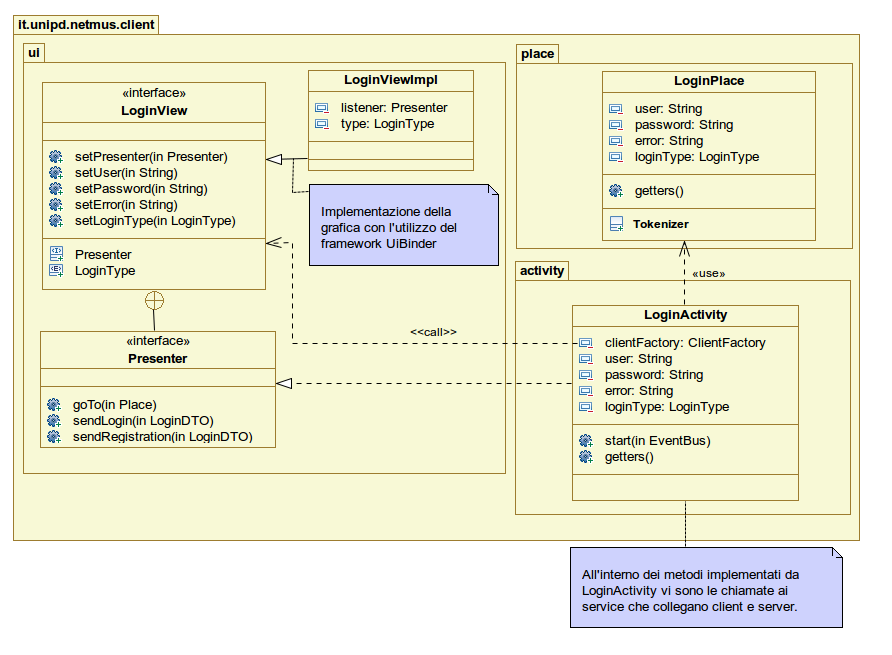
\includegraphics[width=16cm]{img/DP/package.png}
\caption{Diagramma UML delle classi che descrive le dipendenze
fondamentali presenti all'interno del package client.}
\end{figure}
Come possiamo vedere dal diagramma delle classi, la dichiarazione dei metodi
necessari alla comunicazione tra view e model viene fatta nell'interfaccia 
\co{Presenter} innestata nell'interfaccia \co{LoginView}. Cos\`i \co{LoginView}
si prende carico della definizione del presenter, anche se l'implementazione sta
nella classe \co{LoginActivity}, creando una forte dipendenza tra le componenti view e
presenter ma con il vantaggio di rimuovere qualsiasi tipo di collegamento
diretto dell'interfaccia grafica con il model.\\
La parte di visualizzazione vera e propria dei dati risiede in
\co{LoginViewImpl} che viene caricata con il deferred binding all'avvio
dell'applicazione garantendo buona separazione tra parte grafica e parte logica
e di conseguenza buona estendibilit\`a.\\
Questo schema di classi gestisce
anche la funzione di mantenimento dello stato lato client grazie a
\co{LoginPlace}. La classe Place mantiene alcune informazioni per definire lo
stato corrente e le rende disponibili, fornendo metodi \emph{get}, ad ogni
Activity che fa avviare. L'Activity a sua volta pu\`o inviarle, chiamando i
metodi \emph{set}, alla View che completa cos\`i il ciclo necessario al
mantenimento dello stato in ogni componente impiegata per la costruzione delle pagine.

\subsection*{Tipo, obiettivo e funzione del componente} % LASCIARE WARNING
Il package \emph{client} rappresenta la parte del sistema con la quale l'utente
pu\`o interagire. Tutte le sue classi ed i suoi sottopackage saranno compilati in
JavaScript da GWT, prima che il sistema venga depositato nel dominio
\emph{appspot.com} di Google. Contiene la classe \underline{Entry Point}
\co{Netmus}.
\subsection*{Relazioni d'uso di altre componenti}
Il package \emph{client} utilizza i DTO nel package \emph{shared}.
\subsection*{Interfacce con e relazioni d'uso da altre componenti}
Nessuna.
\subsection*{Attivit\`a svolte e dati trattati}
Le attivit\`a svolte dalle sue classi verranno qui di seguito descritte.

\subsection{Classe Netmus}
\subsubsection*{Requisiti obbligatori soddisfatti}
\begin{itemize}
	\item C1FN-1 Web Application Netmus
\end{itemize}
\subsubsection*{Tipo, obiettivo e funzione del componente}
Questa classe rappresenta l'Entry Point di GWT che genera tutte le altre
componenti e rende disponibile e visibile l'intero sistema.\\
In particolare andr\`a a creare dinamicamente il \co{ClientFactoryImpl} adatto,
nel caso ce ne fossero diversi, e lo aggancia insieme all'EventBus al nostro
\co{NetmusPlaceHistoryMapper} ed al \co{NetmusActivityMapper}.
Inoltre allaccia al body Html il widget principale dell'applicazione.

\subsubsection*{Relazioni d'uso di altre componenti}
La classe \co{Netmus} utilizza le classi \co{ClientFactory},
\co{NetmusActivityMapper} e \\\co{NetmusPlaceHistoryMapper}.

\subsubsection*{Interfacce con e relazioni d'uso da altre componenti}
Nessuna.

\subsubsection*{Attivit\`a svolte e dati trattati}
\co{Netmus} praticamente si occupa di avviare il sistema e portare l'utente alla
pagina iniziale di Login o, se gi\`a loggato, alla sua pagina Profilo.

\subsection{Classe ClientFactoryImpl (\emph{Abstract Factory})}
\subsubsection*{Requisiti obbligatori soddisfatti}
\begin{itemize}
	\item C1QN-2.3 Portabilit\`a
\end{itemize}
\subsubsection*{Tipo, obiettivo e funzione del componente}
In Netmus \`e disponibile un'unica implementazione dell'interfaccia
\co{ClientFactory}, poich\'e per il momento non \`e contemplato un utilizzo di
alternative all'interfaccia utente desktop.
Nella classe si definiscono le propriet\`a di un vista (desktop) del
sistema.

\subsubsection*{Relazioni d'uso di altre componenti}
La classe utilizza \co{EventBus}, \co{PlaceController}, \co{LoginView},
\co{ProfileView}, \co{EditUserView} e
\co{EditSongView}.
\subsubsection*{Interfacce con e relazioni d'uso da altre componenti}
\co{Netmus} crea l'istanza della classe. L'interfaccia \co{ClientFactory} \`e
utilizzata da \co{ActivityMapper} e successivamente dalle \co{Activity} per
l'utilizzo dell'EventBus.
\subsubsection*{Attivit\`a svolte e dati trattati}
La classe si occupa di istanziare l'event bus, il place controller e le varie
view. L'event bus gestisce le comunicazioni tra componenti, il place
controller permette la navigazione tra i Place e si occupa di avvisare
l'utente prima del passaggio ad uno stato differente.


\newpage
\section{Package client.ui} % LASCIARE WARNING
\subsection*{Requisiti obbligatori soddisfatti}
\begin{itemize}
	\item C1FN-1 Web Application Netmus
	\item C1FN-1.1 Grafica simile ad iTunes
	\item C1FN-1.2 Registrazione
	\item C1QN-2 Utilizzo
\end{itemize}
\subsection*{Tipo, obiettivo e funzione del componente}
Il package \emph{ui} contiene le interfacce e le implementazioni delle View del
sistema. Le View generano gli ambienti grafici (assimilabili all'interfaccia
utente di iTunes) con cui gli utenti possono interagire e si occupano di
catturare gli eventi da essi prodotti.


\subsection*{Relazioni d'uso di altre componenti}
Questo package utilizza \emph{place} per creare istanze dei vari Place quando
richiesto.

\subsection*{Interfacce con e relazioni d'uso da altre componenti}
Viene utilizzato dal package \emph{activity}.

\subsection*{Attivit\`a svolte e dati trattati}
In sostanza svolge il compito di organizzare le informazioni del model in un
interfaccia accessibile dall'utente.

\subsection{Classe LoginView}
\subsubsection*{Requisiti obbligatori soddisfatti}
\begin{itemize}
	\item C1FN-1.2 Registrazione
\end{itemize}
\subsubsection*{Tipo, obiettivo e funzione del componente}
La classe \co{LoginView} rappresenta la finestra di login fornita all'utente
ogni qualvolta questo accede al sistema senza essersi gi\`a autenticato
precedentemente. \`E possibile effettuare la registrazione a NetMus
selezionando l'apposita sezione ed inserendo un nuovo username ed una password
con le relative conferme. La classe \co{LoginViewImpl} implementa l'interfaccia
\co{LoginView} che estende \co{isWidget} (interfaccia introdotta da GWT 2.1)
permettendo l'utilizzo di UiBinder per la disposizione dei widget e la gestione
degli handler. 
\subsubsection*{Relazioni d'uso di altre componenti} Le azioni invocabili
sono tutte definite nell'interfaccia interna
\co{Presenter} e saranno utilizzate all'interno dei metodi handler. Viene
definito un \emph{enum} riguardante la tipologia di login che viene utilizzato
anche da \co{LoginActivity} e \co{LoginPlace}. \\ I contratti dei metodi (che vengono
implementati in \co{LoginActivity}) e l'\emph{enum} in questione sono:
\begin{itemize}
  \item \underline{public void goTo(in Place)} : permette di spostarsi in un
  place differente anche relativo ad un'altra view. Ad esempio per aprire la pagina di
  \co{ProfileView} una volta verificato il login.
  \item \underline{public void sendLogin(in LoginDTO) throws  LoginException}
  : invia al server il login inserito dall'utente e ritorna \emph{true} solamente se viene
  verificato, altrimenti ritorna \emph{false} con la relativa eccezione.
  \item \underline{public void sendRegistration(in LoginDTO) throws
  RegistrationException} : invia al server i dati di registrazione inseriti
  dall'utente e ritorna \emph{true} se sono stati inseriti con successo nel database.
  \item \underline{public enum LoginType \{NETMUSLOGIN, NETMUSREGISTRATION\}} :
  Definisce le tipologie di login e registrazione possibili.
\end{itemize}
Per permettere all'utente di cambiare pagina o stato della finestra la classe
pu\`o istanziare oggetti di tipo \co{LoginPlace}. Il form di login e quello di
registrazione appartengono ad uno stesso stato quindi i \co{LoginPlace}
istanziati saranno relativi a situazioni di errore o di login effettuato con successo. 
\subsubsection*{Interfacce con e relazioni d'uso da altre componenti} La vista
viene creata da \co{ClientFactory} ed \`e settata ed utilizzata dalla
\co{LoginActivity}. 
\subsubsection*{Attivit\`a svolte e dati trattati} La classe permette all'utente
di scegliere se effettuare il login oppure la registrazione attraverso
un'interfaccia grafica accattivante e di semplice utilizzo, contiene una form
per l'inserimento password e nome utente e pu\`o visualizzare warning se i dati
inseriti non sono corretti. \\
Tra gli attributi ed i metodi presentati sono anche i widget e gli handler
implementati con UiBinder in LoginViewImpl.
\begin{longtable}{|p{0.4\textwidth}|p{0.4\textwidth}|}
\hline
\rowcolor{orange} \bo{Attributo} & \bo{Descrizione} \\
\hline
+ myConstants: MyConstants & Gestore dell'internazionalizzazione associato a
questa pagina.\\\hline 
- listener: Presenter & Presenter associato a questa
pagina.\\\hline 
- type: LoginType & Tipologia di accesso che si sta effettuando.\\\hline
@UiField container: HTMLPanel & Finestra che contiene l'intera pagina.\\\hline
@UiField login: Label & Etichetta che se cliccata invia i dati e avvia
la procedura di login o di registrazione.\\\hline 
@UiField register: Label & Etichetta che se cliccata apre la
visualizzazione del form di registrazione.\\\hline 
@UiField account: Label &
Etichetta che descrive i campi di inserimento login e password.\\\hline
@UiField user: TextBox & Campo per l'inserimento del login.\\\hline
@UiField password: TextBox & Campo per l'inserimento della password.\\\hline
@UiField c\_password: TextBox & Campo per l'inserimento della
password di conferma.\\\hline 
@UiField error: Label & Etichetta che contiene il testo di eventuali
errori avvenuti durante il login o la registrazione.\\\hline 
\end{longtable}
\begin{longtable}{|p{0.4\textwidth}|p{0.4\textwidth}|}
\hline
\rowcolor{orange} \bo{Metodo} & \bo{Descrizione} \\
\hline
+ setPresenter(in Presenter) & Questo metodo viene usato da
\co{LoginActivity} per impostare una sua istanza come implementazione
del presenter di \co{LoginView}.\\\hline 
+ setUser(in String) & Questo metodo viene usato da
\co{LoginActivity} per impostare l'username inserito nel precedente
tentativo di login o registrazione.\\\hline 
+ setPassword(in String) & Questo metodo viene usato da
\co{LoginActivity} per impostare la password inserita nel precedente
tentativo di login o registrazione.\\\hline 
+ setError(in String) & Questo metodo viene usato da
\co{LoginActivity} per impostare il testo di un errore occorso nel
precedente tentativo di login o registrazione.\\\hline
+ setLoginType(in LoginType) & Serve ad impostare il tipo di login o
registrazione che si sta effettuando.\\\hline 
\# goRegisterView() & Visualizza i form aggiuntivi necessari alla
registrazione.\\\hline 
@UiHandler(``login'') handleClick(in ClickEvent) & Invia all'activity
associata la richiesta di login o registrazione.\\\hline
@UiHandler(``register'') handleClick(in ClickEvent) & Se la pagina si
trova nello stato \co{LoginType.LOGINNETMUS} ridispone gli elementi in
modo da visualizzare il form intero per la registrazione, altrimenti
nasconde i campi per registrazione lasciando solamente quelli per il
login.\\\hline
\end{longtable}

\subsection{Classe ProfileView}
\subsubsection*{Requisiti obbligatori soddisfatti}
\begin{itemize}
	\item C1FN-1.1.1 Brani elencati opportunamente
	\item C1FN-1.1.3 Visualiz. info dettagliate dei brani
\end{itemize}
\subsubsection*{Tipo, obiettivo e funzione del componente}
Il sistema mette a disposizione una vista per la visualizzazione del profilo e
dei brani di un generico utente registrato e per la riproduzione dalla musica
tramite un player streaming. La classe \co{ProfileViewImpl} implementa
l'interfaccia \co{ProfileView} che estende \co{isWidget} (interfaccia introdotta
da GWT 2.1).
\subsubsection*{Relazioni d'uso di altre componenti} 
La classe istanzia oggetti di tipo \co{ProfilePlace} che definiscono gli stati
attuali della vista.
\subsubsection*{Interfacce con e relazioni d'uso da altre componenti}
 La vista viene creata da \co{ClientFactory} ed \`e settata ed utilizzata dalla
 \co{ProfileActivity}.
 \subsubsection*{Attivit\`a svolte e dati trattati}
Contiene la lista dei profili che l'utente pu\`o visualizzare e gli strumenti
per navigare tra i cataloghi musicali.

\subsection{Classe EditUserView}
\subsubsection*{Requisiti obbligatori soddisfatti}
\begin{itemize}
	\item C1FN-1.4 Gestione profilo personale
	\item C1FN-1.4.1 Modifica informazioni personali
	\item C1FN-1.4.2 Cambio password
	\item C1FN-1.4.3 Cancellazione del proprio account
\end{itemize}
\subsubsection*{Tipo, obiettivo e funzione del componente}
Il sistema mette a disposizione una vista per la
modifica delle informazioni \subsection{Classe ProfileView}
\subsubsection*{Requisiti obbligatori soddisfatti}
\begin{itemize}
   \item C1FN-1.1.1 Brani elencati opportunamente
   \item C1FN-1.1.3 Visualiz. info dettagliate dei brani
\end{itemize}
\subsubsection*{Tipo, obiettivo e funzione del componente}
Il sistema mette a disposizione una vista per la visualizzazione del profilo e
dei brani di un generico utente registrato e per la riproduzione dalla musica
tramite un player streaming. La classe \co{ProfileViewImpl} implementa
l'interfaccia \co{ProfileView} che estende \co{isWidget} (interfaccia introdotta
da GWT 2.1).
\subsubsection*{Relazioni d'uso di altre componenti} 
La classe istanzia oggetti di tipo \co{ProfilePlace} che definiscono gli stati
attuali della vista.
\subsubsection*{Interfacce con e relazioni d'uso da altre componenti}
 La vista viene creata da \co{ClientFactory} ed \`e settata ed utilizzata dalla
 \co{ProfileActivity}.
 \subsubsection*{Attivit\`a svolte e dati trattati}
Contiene la lista dei profili che l'utente pu\`o visualizzare e gli strumenti
per navigare tra i cataloghi musicali.

\subsection{Classe EditUserView}
\subsubsection*{Requisiti obbligatori soddisfatti}
\begin{itemize}
   \item C1FN-1.4 Gestione \subsection{Classe ProfileView}
\subsubsection*{Requisiti obbligatori soddisfatti}
\begin{itemize}
   \item C1FN-1.1.1 Brani elencati opportunamente
   \item C1FN-1.1.3 Visualiz. info dettagliate dei brani
\end{itemize}
\subsubsection*{Tipo, obiettivo e funzione del componente}
Il sistema mette a disposizione una vista per la visualizzazione del profilo e
dei brani di un generico utente registrato e per la riproduzione dalla musica
tramite un player streaming. La classe \co{ProfileViewImpl} implementa
l'interfaccia \co{ProfileView} che estende \co{isWidget} (interfaccia introdotta
da GWT 2.1).
\subsubsection*{Relazioni d'uso di altre componenti} 
La classe istanzia oggetti di tipo \co{ProfilePlace} che definiscono gli stati
attuali della vista.
\subsubsection*{Interfacce con e relazioni d'uso da altre componenti}
 La vista viene creata da \co{ClientFactory} ed \`e settata ed utilizzata dalla
 \co{ProfileActivity}.
 \subsubsection*{Attivit\`a svolte e dati trattati}
Contiene la lista dei profili che l'utente pu\`o visualizzare e gli strumenti
per navigare tra i cataloghi musicali.

\subsection{Classe EditUserView}
\subsubsection*{Requisiti obbligatori soddisfatti}
\begin{itemize}
   \item C1FN-1.4 Gestione profilo personale
   \item C1FN-1.4.1 Modifica informazioni personali
   \item C1FN-1.4.2 Cambio password
   \item C1FN-1.4.3 Cancellazione del proprio account
\end{itemize}
\subsubsection*{Tipo, obiettivo e funzione del componente}
Il sistema mette a disposizione una vista per la
modifica delle informazione profilo personale
   \item C1FN-1.4.1 Modifica informazioni personali
   \item C1FN-1.4.2 Cambio password
   \item C1FN-1.4.3 Cancellazione del proprio account
\end{itemize}
\subsubsection*{Tipo, obiettivo e funzione del componente}
Il sistema mette a disposizione una vista per la
modifica delle informazioni personali dell'utente registrato. La classe
\co{EditUserViewImpl} implementa l'interfaccia \co{EditUserView} che estende
\co{isWidget} (interfaccia introdotta da GWT 2.1).

\subsubsection*{Relazioni d'uso di altre componenti}
La classe istanzia oggetti di tipo \co{EditUserPlace} che definiscono gli stati
attuali della vista.
\subsubsection*{Interfacce con e relazioni d'uso da altre componenti}
La vista viene creata da \co{ClientFactory} ed \`e settata ed utilizzata dalla
\co{EditUserActivity}.
\subsubsection*{Attivit\`a svolte e dati trattati}
Mette a disposizione gli strumenti per la modifica delle informazioni personali
dell'utente registrato (cambio password, cancellazione account,
pubblicazione catalogo)

\newpage
\section{Package client.activity} % LASCIARE WARNING
\subsection*{Requisiti obbligatori soddisfatti}
\begin{itemize}
	\item C1FN-1 WEB Application NetMus
\end{itemize}
\subsection*{Tipo, obiettivo e funzione del componente}
Questo package contiene le classi Activity che corrispondono in pratica alla
componente Presenter del pattern MVP originale. la Activity sono avviate e
terminate da un ActivityManager associato con un contenitore Widget. Un activity
pu\`o inoltre visualizzare automaticamente un avviso quando sta per essere
terminata (in pi\`u l'ActivityManager ci avvisa quando la finestra sta per
essere chiusa).

\subsection*{Relazioni d'uso di altre componenti} Il package usa gli oggetti
View di \emph{ui} e Place di \emph{place} per gestire informazioni di stato o
modificatori della vista, ma quando serve pu\`o utilizzare servizi forniti da
\emph{service} (per passare i dati alla view).
\subsection*{Interfacce con e relazioni d'uso da altre componenti} Le istanze
delle classi Activity vengono create dal \co{NetmusActivityMapper} che quando,
riceve una richiesta di una Activity, ritorna una corretta istanza di tale
classe, in base al Place corrente.
\subsection*{Attivit\`a svolte e dati trattati} Il package \emph{activity} si
pu\`o considerare il boss, poich\'e gestisce l'intera logica di business del
client.

\subsection{Classe LoginActivity}
\subsubsection*{Requisiti obbligatori soddisfatti}
\begin{itemize}
	\item C1FN-1.2 Registrazione
\end{itemize}
\subsubsection*{Tipo, obiettivo e funzione del componente}
Questa classe \`e di tipo \co{AbstractActivity}, implementa il \co{Presenter}
interno alla \co{LoginView} rappresentando quindi il collegamento tra la parte
grafica presente nel client ed il modello che risiede nel server.
\subsubsection*{Relazioni d'uso di altre componenti} Invoca i servizi
asincroni di autenticazione forniti da \co{LoginService}.\\ Si occupa di
recuperare i dati da \co{LoginPLace} e trasferirli alla \co{LoginView}. 
\subsubsection*{Interfacce con e relazioni d'uso da altre componenti} 
Viene creata da \co{NetmusActivityMapper} quando viene richiesta la Activity da
un Place di tipo \co{LoginPlace}.
\subsubsection*{Attivit\`a svolte e dati trattati}
Questa classe ha il compito di settare gli attributi della pagina di login
adeguatamente allo stato rappresentato dal \co{LoginPlace} che l'ha originata e
deve fornire inoltre l'implementazione dei metodi dichiarati dalla view
all'interno dell'interfaccia \co{Presenter}.
\begin{longtable}{|p{0.4\textwidth}|p{0.4\textwidth}|}
\hline
\rowcolor{orange} \bo{Attributo} & \bo{Descrizione} \\
\hline
- user: String & Username inserito dall'utente nello stato corrente, sar\`a
inizializzato con il valore ricevuto dal \co{LoginPlace} nel
costruttore.\\\hline 
- password: String & Password inserita dall'utente nello stato corrente, sar\`a
inizializzata con il valore ricevuto dal \co{LoginPlace} nel
costruttore.\\\hline 
- error: String & Errore pi\`u rilevante occorso nello stato
corrente, sar\`a inizializzato con il valore ricevuto dal \co{LoginPlace} nel
costruttore.\\\hline
- loginType: LoginType & Tipologia di login o registrazione che si sta
effettuando nello stato corrente, sar\`a
inizializzato con il valore ricevuto dal \co{LoginPlace} nel
costruttore.\\\hline
+ LoginType NETMUSLOGIN, NETMUSREGISTRATION: enum & attributo ereditato
da \co{LoginView.Presenter}\\\hline
\end{longtable}
\begin{longtable}{|p{0.4\textwidth}|p{0.4\textwidth}|}
\hline
\rowcolor{orange} \bo{Metodo} & \bo{Descrizione} \\
\hline
+ start(AcceptsOneWidget, EventBus) & Invocato da \co{ActivityManager}
per avviare una nuova \co{LoginActivity}\\\hline 
+ goTo(in Place) & Permette di
spostarsi in un place differente anche relativo ad un'altra view. Ad esempio per aprire la pagina di
\co{ProfileView} una volta verificato il login. Verr\`a quindi
richiamato sempre al termine dei metodi \co{sendLogin} e
\co{sendRegistration}\\\hline 
+ sendLogin(in LoginDTO) & Invia al
server il login inserito dall'utente dopo averne controllato la validit\`a
(e-mail valida, password sufficientemente lunga). Se la richiesta di
autenticazione al server ha successo il metodo avvia la sessione HTTP ed apre la
pagina principale \co{ProfileView}, se invece la comunicazione col
server fallisce o non sono stati superati i controlli di validit\`a del
login il metodo apre un'altra finestra di login con il messaggio di
errore adeguato. Gli errori lato server vengono gestiti con eccezioni di
tipo \co{LoginException}.\\\hline 
+ sendRegistration(in LoginDTO) & Invia al
server i dati di registrazione inseriti dall'utente dopo averne controllato la
correttezza (e-mail valida, password sufficientemente lunga). Se la
risposta del server è affermativa ed i dati sono stati inseriti con
successo l'utente viene indirizzato alla pagina di \co{ProfileView},
altrimenti il metodo apre un'altra finestra di login con il messaggio di
errore adeguato. Gli errori lato server vengono gestiti con eccezioni di
tipo \co{RegistrationException}.\\\hline
\end{longtable}


\subsection{Classe ProfileActivity}
\subsubsection*{Requisiti obbligatori soddisfatti}
\begin{itemize}
	\item C1FN-1.1.1 Brani elencati opportunamente
	\item C1FN-1.1.3 Visualiz. info dettagliate dei brani
\end{itemize}
\subsubsection*{Tipo, obiettivo e funzione del componente}
Questa classe estende \co{AbstractActivity}, implementa il \co{Presenter}
interno alla \co{ProfileView} e richiede al \co{clientFactory} di
implementarela.
\subsubsection*{Relazioni d'uso di altre componenti}
Invoca i servizi di interrogazione e modifica dei dati profilo forniti da
\co{UsersService} e utilizza le relative classi \co{ProfilePlace} e
\co{ProfileView}.
\subsubsection*{Interfacce con e relazioni d'uso da altre componenti}
Viene creata da \co{NetmusActivityMapper} quando viene richiesta la Activity da
un Place di tipo \co{ProfilePlace}.
\subsubsection*{Attivit\`a svolte e dati trattati}
Questa classe gestisce, assieme a \co{UsersService}, le attivit\`a utili alla
creazione ed interazione con l'utente della pagina principale come la
richiesta dei dati utente dettagliati, della lista dei brani, del dettaglio di
un brano, ecc.


\subsection{Classe EditUserActivity}
\subsubsection*{Requisiti obbligatori soddisfatti}
\begin{itemize}
	\item C1FN-1.4 Gestione profilo personale
	\item C1FN-1.4.1 Modifica informazioni personali
	\item C1FN-1.4.2 Cambio password
	\item C1FN-1.4.3 Cancellazione del proprio account
\end{itemize}
\subsubsection*{Tipo, obiettivo e funzione del componente}
Questa classe estende \co{AbstractActivity}, implementa il \co{Presenter}
interno alla \co{EditUserView} e richiede al \co{clientFactory} di
implementarela.
\subsubsection*{Relazioni d'uso di altre componenti}
Invoca i servizi di interrogazione e modifica dei dati profilo forniti da
\co{UsersService} e utilizza le relative classi \co{EditUserPlace} e
\co{EditUserView}.
\subsubsection*{Interfacce con e relazioni d'uso da altre componenti}
Viene creata da \co{NetmusActivityMapper} quando viene richiesta la Activity da
un Place di tipo \co{EditUserPlace}.
\subsubsection*{Attivit\`a svolte e dati trattati}
Questa classe gestisce, assieme a \co{UsersService}, le attivit\`a utili alla
modifica delle informazioni personali visualizzate nel profilo.

\newpage
\section{Package client.place} % LASCIARE WARNING
\subsection*{Requisiti obbligatori soddisfatti}
\begin{itemize}
	\item C1FN-1 WEB Application NetMus
\end{itemize}
\subsection*{Tipo, obiettivo e funzione del componente}
Il package contiene le classi di tipo Place. I Place sono indispensabili
per far s\`i che la corrispondente Activity sia accessibile via URL e per
memorizzare i dati relativi allo stato corrente del sistema in modo che siano
rapidamente recuperabili. 
\subsection*{Relazioni d'uso di altre componenti} A
questo package appartengono le classi \co{LoginPlace}, \co{ProfilePlace},
\co{EditUserPlace}, \\\co{EditSongsPlace}.\\
In ognuna di queste classi \`e presente una sottoclasse \co{Tokenizer} che
permette di serializzare lo stato del Place in un simbolo (token) URL e che non
\`e implementata da noi ma dal framework che utilizziamo, per questo non sar\`a
specificata nelle liste di attributi delle classi di questo package.
\subsection*{Interfacce con
e relazioni d'uso da altre componenti} I suoi elementi vengono utilizzati dal package \emph{mvp}. 
\subsection*{Attivit\`a svolte e dati trattati} Organizza i Places.

\subsection{Classe LoginPlace}
\subsubsection*{Requisiti obbligatori soddisfatti}
\begin{itemize}
	\item C1FN-1.2 Registrazione
\end{itemize}
\subsubsection*{Tipo, obiettivo e funzione del componente}
\co{LoginPlace} estende la classe \co{Place} messa a disposizione da GWT. La
classe \`e associata alla classe interna \co{Tokenizer} che permette di
serializzare lo stato del Place in un simbolo (token) URL.
Ha la funzione di contenere i dati dello stato corrente della pagina di login.
\subsubsection*{Relazioni d'uso di altre componenti}
Nessuna.
\subsubsection*{Interfacce con e relazioni d'uso da altre componenti}
La classe \`e creata da \co{LoginView} quando viene effettuato un qualsiasi
tentativo di login o registrazione ed \`e utilizzata nella creazione della
conseguente \co{LoginActivity}. 
\subsubsection*{Attivit\`a svolte e dati trattati} Il compito della classe \`e
quello di indicizzare gli stati della pagina di login e mantenerne i dati
finch\'e l'applicazione \`e attiva. Questo permette inoltre di rendere
accessibili le funzionalit\`a di history e bookmarking del browser.
\begin{longtable}{|p{0.4\textwidth}|p{0.4\textwidth}|}
\hline
\rowcolor{orange} \bo{Attributo} & \bo{Descrizione} \\
\hline
- user: String & Username inserito dall'utente nello stato corrente, sar\`a
diverso da \emph{null} solo nel caso vi si acceda in seguito ad un errore o
dalla history.\\\hline 
- password: String & Password inserita dall'utente nello stato corrente, sar\`a
diversa da \emph{null} solo nel caso vi si acceda in seguito ad un errore o
dalla history.\\\hline 
- error: String & Errore pi\`u rilevante occorso nello stato
corrente, sar\`a diverso da \emph{null} solo nel caso sia avvenuto un
errore nel tentativo di login/registrazione precedente.\\\hline
- loginType: LoginType & Tipologia di login o registrazione che si sta
effettuando nello stato corrente, di default \`e NETMUSLOGIN.\\\hline
\end{longtable}
\begin{longtable}{|p{0.4\textwidth}|p{0.4\textwidth}|}
\hline
\rowcolor{orange} \bo{Metodo} & \bo{Descrizione} \\
\hline
+ getUser() : String & Getter dell'attributo \co{user}\\\hline
+ getPassword() : String & Getter dell'attributo \co{password}\\\hline
+ getError() : String & Getter dell'attributo \co{error}\\\hline
+ getLoginType() : LoginType & Getter dell'attributo \co{loginType}\\\hline
\end{longtable}

\subsection{Classe ProfilePlace}
\subsubsection*{Requisiti obbligatori soddisfatti}
\begin{itemize}
	\item C1FN-1.1.1 Brani elencati opportunamente
	\item C1FN-1.1.3 Visualiz. info dettagliate dei brani
\end{itemize}
\subsubsection*{Tipo, obiettivo e funzione del componente}
\co{ProfilePlace} estende la classe \co{Place} messa a disposizione da GWT. La
classe \`e associata alla classe interna \co{Tokenizer} che permette di
serializzare lo stato del Place in un simbolo (token) URL.
\subsubsection*{Relazioni d'uso di altre componenti}
Nessuna.
\subsubsection*{Interfacce con e relazioni d'uso da altre componenti}
La classe \`e creata da \co{ProfileView} utilizzata da \co{ProfileActivity}.
\subsubsection*{Attivit\`a svolte e dati trattati}
Il compito della classe \`e quello di indicizzare gli stati di
\co{ProfileActivity} in modo da rendere accessibili le funzionalit\`a di history
e bookmarking del browser.

\subsection{Classe EditUserPlace}
\subsubsection*{Requisiti obbligatori soddisfatti}
\begin{itemize}
	\item C1FN-1.4 Gestione profilo personale
	\item C1FN-1.4.1 Modifica informazioni personali
	\item C1FN-1.4.2 Cambio password
	\item C1FN-1.4.3 Cancellazione del proprio account
\end{itemize}
\subsubsection*{Tipo, obiettivo e funzione del componente}
\co{EditUserPlace} estende la classe \co{Place} messa a disposizione da GWT. La
classe \`e associata alla classe interna \co{Tokenizer} che permette di
serializzare lo stato del Place in un simbolo (token) URL.
\subsubsection*{Relazioni d'uso di altre componenti}
Nessuna.
\subsubsection*{Interfacce con e relazioni d'uso da altre componenti}
La classe \`e creata da \co{EditUserView} utilizzata da \co{EditUserActivity}.
\subsubsection*{Attivit\`a svolte e dati trattati}
Il compito della classe \`e quello di indicizzare gli stati di
\co{EditUserActivity} in modo da rendere accessibili le funzionalit\`a di
history e bookmarking del browser.

\newpage
\section{Package client.mvp} % LASCIARE WARNING
\subsection*{Requisiti obbligatori soddisfatti}
\begin{itemize}
	\item C1FN-1 WEB Application NetMus
\end{itemize}
\subsection*{Tipo, obiettivo e funzione del componente}
Il package contiene le classi funzionali al meccanismo delle Activity e dei
Places.
\subsection*{Relazioni d'uso di altre componenti}
Fanno parte di questo package le classi \co{NetmusHistoryMapper} e
\co{NetmusActivityMapper}.
\subsection*{Interfacce con e relazioni d'uso da altre componenti}
Nessuna.
\subsection*{Attivit\`a svolte e dati trattati}
Le attivit\`a svolte dalle sue classi verranno qui di seguito descritte.

\subsection{Classe NetmusActivityMapper}
\subsubsection*{Requisiti obbligatori soddisfatti}
\begin{itemize}
	\item C1FN-1 WEB Application NetMus
\end{itemize}
\subsubsection*{Tipo, obiettivo e funzione del componente}
Questa classe si occupa di mappare ogni attivit\`a con il corrispondente Place.
\subsubsection*{Relazioni d'uso di altre componenti}
La classe utilizza istanze di classi appartenenti al package
\emph{client.place} e crea istanze di classi appartenenti al package
\emph{client.activity}.
\subsubsection*{Interfacce con e relazioni d'uso da altre
componenti} Nessuna.
\subsubsection*{Attivit\`a svolte e dati trattati}
Tramite un riferimento ad un Place crea e restituisce un oggetto activity.

\subsection{Classe NetmusPlaceHistoryMapper}
\subsubsection*{Requisiti obbligatori soddisfatti}
\begin{itemize}
	\item C1FN-1 WEB Application NetMus
\end{itemize}
\subsubsection*{Tipo, obiettivo e funzione del componente}
Dichiara e riferisce tutti i places che saranno utilizzati da Netmus.
\subsubsection*{Relazioni d'uso di altre componenti}
Utilizza i PlaceTokenizer.
\subsubsection*{Interfacce con e relazioni d'uso da altre componenti}
Il PlaceHistoryHandler utilizza la classe per la sincronizzazione del URL.
\subsubsection*{Attivit\`a svolte e dati trattati}
Funge da connessione tra i PlaceTokenizer (classe interna ad ogni Place) e il
PlaceHistoryHandler (messo a disposizione da GWT) che sincronizza l'URL del
browser con i vari Place.

\newpage
\section{Package client.service} % LASCIARE WARNING
\subsection*{Requisiti obbligatori soddisfatti}
\begin{itemize}
	\item C2QN-3.2 Utilizzo della connessione
	\item C1QN-1.9.6 Gestione concorrenza
\end{itemize}
\subsection*{Tipo, obiettivo e funzione del componente}
Il contenuto di questo package \`e di fondamentale importanza poich\'e
rappresenta la parte client del framework RPC che viene utilizzato per scambio
di oggetti tra client e server. \co{client.service} \`e costituito da tutte
le interfacce dei servizi remoti offerti dal server. Le funzionalit\`a delle
classi in esso contenute saranno divise in base al tipo di servizio offerto. Per
ognuno di questi sar\`a presente un'interfaccia normale (che estende
\co{RemoteService}) e un'interfaccia \bo{asincrona}.

\subsection*{Relazioni d'uso di altre componenti}
Queste interfacce vengono implementate su \emph{server}, perci\`o non
hanno relazioni d'uso definite. Verranno sempre usati oggetti DTO (definiti in
\emph{shared}) come pacchetti di scambio nei servizi tra \emph{client} e
\emph{server}.

\subsection*{Interfacce con e relazioni d'uso da altre componenti}
Verranno istanziati degli oggetti di \emph{service} col metodo del
\emph{deferred binding} dalla classe di Entry Point \co{Netmus}, pur avendo
visibilit\`a solamente delle interfacce. Verranno poi usati dalle varie Activity.

\subsection*{Attivit\`a svolte e dati trattati}
Vengono forniti tutti i servizi che il server sar\`a in grado di dare, i dati
trattati saranno i DTO definiti nel package \emph{shared}.

\subsection{Interfaccia SongsService (e SongServiceAsync)}
\subsubsection*{Requisiti obbligatori soddisfatti}
\begin{itemize}
	\item C1FN-1.1.3 Visualiz. info dettagliate dei brani
	\item C1FN-1.9 Ricezione ed elaborazione dei brani
	\item C1FN-1.9.1 Controllo di validit\`a dei dati
	\item C1FN-1.9.5 Inserimento nel Database
	\item C2FN-3.1 Invio delle informazioni
\end{itemize}
\subsubsection*{Tipo, obiettivo e funzione del componente}
Questa classe dovr\`a consentire alle componenti Activity di \emph{client} di
inviare richieste di vario tipo a \emph{server} riguardanti informazioni sui
brani musicali. Sar\`a presente anche \co{SongServiceAsync}, che gestir\`a il ritorno
dai metodi in maniera asincrona.

\subsubsection*{Relazioni d'uso di altre componenti}
Queste interfacce verranno implementate su \emph{server}, perci\`o non
avranno relazioni d'uso definite, se non con gli oggetti DTO
(\co{UserDTO, SongDTO}, \co{SongSummaryDTO}, \co{MusicLibraryDTO}) che verranno
utilizzati per il trasferimento client-server.

\subsubsection*{Interfacce con e relazioni d'uso da altre componenti}
Questa interfaccia verr\`a istanziata da \co{Netmus} tramite deferred
binding e verr\`a utilizzata da \co{ProfileActivity} ed \co{EditSongsActivity}.

\subsubsection*{Attivit\`a svolte e dati trattati}
Questa interfaccia fornir\`a l'accesso a servizi per richiedere qualsiasi tipo
di informazione riguardante i brani musicali e utilizzer\`a dati di tipo SongDTO
e SongSummaryDTO.

\subsection{Interfaccia UsersService (e UsersServiceAsync)}
\subsubsection*{Requisiti obbligatori soddisfatti}
\begin{itemize}
	\item C1FN-1.4 Gestione profilo personale
	\item C1FN-1.4.1 Modifica informazioni personali
	\item C1FN-1.4.2 Cambio password
	\item C1FN-1.4.3 Cancellazione del proprio account
\end{itemize}
\subsubsection*{Tipo, obiettivo e funzione del componente}
Questa classe consentir\`a alle componenti Activity di \emph{client} di inviare
richieste di vario tipo a \emph{server} riguardanti le informazioni personali
dell'utente da mostrare  nell'interfaccia grafica. Sar\`a presente anche
\co{UsersServiceAsync}, che gestir\`a il ritorno dai metodi in maniera asincrona.

\subsubsection*{Relazioni d'uso di altre componenti}
Queste interfacce verranno implementate su \emph{server}, perci\`o non
avranno relazioni d'uso definite, se non con gli oggetti DTO (\co{UserDTO},
\co{UserSummaryDTO}, \co{UserCompleteDTO}) che verranno utilizzati per il
trasferimento client-server.

\subsubsection*{Interfacce con e relazioni d'uso da altre componenti}
Questa interfaccia verr\`a istanziata da \co{Netmus} tramite deferred
binding e verr\`a utilizzata da \co{EditUserActivity} e \co{ProfileActivity}.

\subsubsection*{Attivit\`a svolte e dati trattati}
Questa interfaccia fornir\`a l'accesso a servizi per richiedere o
modificare (quando possibile) qualsiasi tipo di informazione riguardante gli
utenti del sistema e utilizzer\`a dati di tipo \co{UserDTO}, \co{UserSummaryDTO}
e \co{UserCompleteDTO}.

\subsection{Interfaccia LibraryService (e LibraryServiceAsync)}
\subsubsection*{Requisiti obbligatori soddisfatti}
\begin{itemize}
	\item C1FN-1.1.1 Brani elencati opportunamente
\end{itemize}
\subsubsection*{Tipo, obiettivo e funzione del componente}
Questa classe consentir\`a alle componenti Activity di \emph{client} di inviare
richieste di vario tipo a \emph{server} riguardanti il catalogo musicale utente
da mostrare nell'interfaccia grafica. Sar\`a presente anche
\co{LibraryServiceAsync}, che gestir\`a il ritorno dai metodi in maniera
asincrona.
\subsubsection*{Relazioni d'uso di altre componenti}
Queste interfacce verranno implementate su \emph{server}, perci\`o non
avranno relazioni d'uso definite, se non con gli oggetti DTO
(\co{MusicLibraryDTO}) che verranno utilizzati per il trasferimento
client-server.
\subsubsection*{Interfacce con e relazioni d'uso da altre componenti}
Questa interfaccia verr\`a istanziata da \co{Netmus} tramite deferred
binding e verr\`a utilizzata da \co{ProfileActivity}.
\subsubsection*{Attivit\`a svolte e dati trattati}
Questa interfaccia fornir\`a l'accesso a servizi per richiedere qualsiasi tipo
di informazione riguardante la libreria musicale utente e utilizzer\`a dati di
tipo \co{MusicLibraryDTO}.


\subsection{Interfaccia LoginService (e LoginServiceAsync)}
\subsubsection*{Requisiti obbligatori soddisfatti}
\begin{itemize}
	\item C1FN-1.2 Registrazione
\end{itemize}
\subsubsection*{Tipo, obiettivo e funzione del componente}
\co{LoginService} mette a disposizione metodi
che soddisfano le possibili richieste verso la parte model riguardanti l'autenticazione degli utenti.
Questi metodi si occupano inoltre di gestire la parte relativa alle sessioni HTTP. 
\`E presente anche \co{LoginServiceAsync}, che gestisce il ritorno dai
metodi in maniera asincrona.

\subsubsection*{Relazioni d'uso di altre componenti}
Queste interfacce vengono implementate su \emph{server}, perci\`o non
hanno relazioni d'uso definite, se non con oggetti \co{LoginDTO} che
vengono utilizzati per il trasferimento client-server.

\subsubsection*{Interfacce con e relazioni d'uso da altre componenti}
Questa interfaccia verr\`a istanziata da \co{Netmus} tramite deferred
binding e viene utilizzata \\\co{LoginActivity} e dalle altre Activity che
permetteranno il login ed il logout dell'utente.

\subsubsection*{Attivit\`a svolte e dati trattati}
Questa interfaccia fornisce l'accesso a servizi per richiedere qualsiasi tipo
di informazione riguardante l'autenticazione dell'utente al sistema
e utilizza dati di tipo \co{LoginDTO}.
Gli attributi e i metodi di questa interfaccia verranno descritti nel
dettaglio nella classe \co{LoginServiceImpl} che li implementa. 

\newpage
%--------------- FORSE -------------------------------
\section{Package client.applet} % LASCIARE WARNING
\subsection*{Requisiti obbligatori soddisfatti}
\begin{itemize}
	\item C2QN-4 Utilizzo
	\item C2FN-3.1 Invio delle informazioni
	\item C2FN-1.5 File ignorati
	\item C2FN-1.2 Recupero manuale
	\item C2FN-1.1 Recupero automatico
	\item C2FN-1 Recupero delle informazioni
\end{itemize}
\subsection*{Obiettivo e funzione del componente}
Questo package conterr\`a le classi necessarie a gestire richieste e segnali
provenienti dalla applet precompilata, che andremo ad inserire nel programma.
Tale applet avr\`a la funzione di effettuare la scansione e l'estrazione
automatica dei tag dei file musicali Mp3, presenti nei dispositivi di
archiviazione di massa che vengono collegati alla macchina dell'utente.\\
Per comunicare con tale applet sono state valutate due possibili metodologie
d'implementazione: l'uso di una libreria che crea un sistema proxy tra la applet
e GWT oppure l'utilizzo di \underline{JSNI} (JavaScript Native Interface) che
sostanzialmente ci permetterebbe di fare chiamate da JavaScript al codice
\underline{Java} e viceversa.

\subsection*{Meccanismo di lavoro del componente}
Una volta ricevuta una richiesta da parte della applet, verr\`a gestita da un
Service che si occuper\`a di elaborare i dati col supporto del server, per poi
notificare all'utente l'avvenuta estrazione e fargliela valutare e accettare.
Una volta accettata la lista brani, si richiede la memorizzazione nel DataStore
tramite \co{SongsService}.

%-----------------------------------------------------

\newpage
\section{Package server}
\subsection*{Requisiti obbligatori soddisfatti}
\begin{itemize}
	\item C1FN-1 WEB Application NetMus
	\item C1QN-1.9.6 Gestione concorrenza
\end{itemize}
\subsection*{Tipo, obiettivo e funzione del componente} % LASCIARE WARNING
Questo package racchiude tutte le classi che collaborano al fine di gestire la
business logic del sistema, ovvero tutte quelle operazioni che potranno essere
compiute sui dati raccolti. Contiene inoltre delle classi di interfacciamento
con il DataStore stesso che consentono il controllo sulla persistenza dei dati.

\subsection*{Relazioni d'uso di altre componenti}
Si fa utilizzo delle classi presenti nel package \emph{shared} in cui vengono
incapsulati tutti i dati in uscita del server.

\subsection*{Interfacce con e relazioni d'uso da altre componenti}
Il package \emph{server} si interfaccia direttamente con \emph{shared} e tramite
questo e con la presenza del package \emph{service} si interfaccia anche con
\emph{client}.

\subsection*{Attivit\`a svolte e dati trattati}
Le attivit\`a svolte dalle sue classi verranno qui di seguito descritte.

\subsection{Classe SongsServiceImpl}
\subsubsection*{Requisiti obbligatori soddisfatti}
\begin{itemize}
	\item C1FN-1.1.3 Visualiz. info dettagliate dei brani
	\item C1FN-1.9 Ricezione ed elaborazione dei brani
	\item C1FN-1.9.1 Controllo di validit\`a dei dati
	\item C1FN-1.9.2 Completamento info da database interno
	\item C1FN-1.9.5 Inserimento nel Database
	\item C2FN-3.1 Invio delle informazioni
\end{itemize}
\subsubsection*{Tipo, obiettivo e funzione del componente}
Questa classe corrisponde all'implementazione del \co{SongsService} (di
\emph{client}) ed estende la classe \co{RemoteServiceServlet}.

\subsubsection*{Relazioni d'uso di altre componenti}
Oltre ad utilizzare ovviamente i DTO in \emph{shared}, verranno creati,
immagazzinati oppure usati i relativi oggetti \emph{persistent}.
Potranno essere usati opportuni servizi \emph{servlet} per andare a prelevare
informazioni sui brani da servizi esterni oppure per cercare il corrispettivo
link di streaming audio-video (tipo YouTube).

\subsubsection*{Interfacce con e relazioni d'uso da altre componenti}
Viene usata dal \emph{client} che ne genera un istanza tramite deferred binding,
utilizzando l'interfaccia \co{SongsService}.

\subsubsection*{Attivit\`a svolte e dati trattati}
Descritte nell'interfaccia lato \emph{client}.

\subsection{Classe UsersServiceImpl}
\subsubsection*{Requisiti obbligatori soddisfatti}
\begin{itemize}
	\item C1FN-1.4 Gestione profilo personale
	\item C1FN-1.4.1 Modifica informazioni personali
	\item C1FN-1.4.2 Cambio password
	\item C1FN-1.4.3 Cancellazione del proprio account
\end{itemize}
\subsubsection*{Tipo, obiettivo e funzione del componente}
Questa classe corrisponde all'implementazione del \co{UsersService} (di
\emph{client}) ed estende la classe \co{RemoteServiceServlet}.

\subsubsection*{Relazioni d'uso di altre componenti}
Oltre ad utilizzare ovviamente i DTO in \emph{shared}, verranno creati,
immagazzinati oppure usati i relativi oggetti \emph{persistent}.

\subsubsection*{Interfacce con e relazioni d'uso da altre componenti}
Viene usata dal \emph{client} che ne genera un istanza tramite deferred binding,
utilizzando l'interfaccia \co{UsersService}.

\subsubsection*{Attivit\`a svolte e dati trattati}
Descritte nell'interfaccia lato \emph{client}.

\subsection{Classe LoginServiceImpl}
\subsubsection*{Requisiti obbligatori soddisfatti}
\begin{itemize}
	\item C1FN-1.2 Registrazione
\end{itemize}
\subsubsection*{Tipo, obiettivo e funzione del componente}
Questa classe corrisponde all'implementazione del \co{LoginService} (di
\emph{client}) ed estende la classe \co{RemoteServiceServlet}.
\subsubsection*{Relazioni d'uso di altre componenti}
Utilizzer\`a i DTO in \emph{shared} e utilizzer\`a le \co{HttpSession} per
gestire le sessioni dell'utente e dargli o meno i diritti d'accesso.
Verranno utilizzate funzionalit\`a interne di gestione login definite in
\co{LoginHelper}. 
\subsubsection*{Interfacce con e relazioni d'uso da altre componenti}
Viene usata dal \emph{client} che ne genera un istanza tramite deferred binding,
utilizzando l'interfaccia \co{LoginService}.
\subsubsection*{Attivit\`a svolte e dati trattati}
Implementa la parte server delle procedure di login come la verifica della
correttezza della password e l'adeguata
impostazione delle sessioni HTTP.
\begin{longtable}{|p{0.4\textwidth}|p{0.4\textwidth}|}
\hline
\rowcolor{orange} \bo{Metodo} & \bo{Descrizione} \\
\hline
+ insertRegistration(LoginDTO) & Inserisce i dati di login
relativi alla registrazione di un nuovo utente nel database. Pu\`o
lanciare eccezioni di tipo \textless= \co{RegistrationException} in caso vi
siano problemi nell'inserimento.\\\hline 
+ verifyLogin(LoginDTO) & Metodo
fondamentale per l'autenticazione che confronta i dati in input con quelli
presenti nel database per verificare se il login \`e valido. Pu\`o
lanciare eccezioni di tipo \textless= \co{LoginException} in caso il controllo
non vada a buon fine.\\\hline 
+ startLogin(LoginDTO) & Racchiude tutte i passi di autenticazione
dell'utente. Utilizza \co{verifyLogin} e si occupa di iniziare la sessione
dell'utente che si \`e autenticato aggiornando anche l'attributo
\co{lastLogin} in \co{UserAccount}.\\\hline 
+ getLoggedInUserDTO():
UserSummaryDTO & Esegue una ricerca della sessione corrente utilizzando i metodi
di \co{LoginHelper} e ritorna, se presenti, le informazioni di base
(\co{UserSummaryDTO}) dell'utente loggato\\\hline 
+ logout() & Invalida l'autenticazione dell'utente che viene rimandato alla pagina di login.\\\hline
\end{longtable}

\subsection{Classe LibraryServiceImpl}
\subsubsection*{Requisiti obbligatori soddisfatti}
\begin{itemize}
	\item C1FN-1.1.1 Brani elencati opportunamente
\end{itemize}
\subsubsection*{Tipo, obiettivo e funzione del componente}
Questa classe corrisponde all'implementazione del \co{LibraryService} (di
\emph{client}) ed estende la classe \co{RemoteServiceServlet}.

\subsubsection*{Relazioni d'uso di altre componenti}
Oltre ad utilizzare ovviamente i DTO in \emph{shared}, verranno creati,
immagazzinati oppure usati i relativi oggetti \emph{persistent}.

\subsubsection*{Interfacce con e relazioni d'uso da altre componenti}
Viene usata dal \emph{client} che ne genera un istanza tramite deferred binding,
utilizzando l'interfaccia \co{LibraryService}.

\subsubsection*{Attivit\`a svolte e dati trattati}
Descritte nell'interfaccia lato \emph{client}.

\subsection{Classe LoginHelper}
\subsubsection*{Requisiti obbligatori soddisfatti}
\begin{itemize}
	\item C1FN-1.2 Registrazione
\end{itemize}
\subsubsection*{Tipo, obiettivo e funzione del componente}
La classe \co{LoginHelper} offre funzionalit\`a statiche
per gestire le sessioni HTML, utili a \co{LoginServiceImpl} ed a
\emph{servlet}.

\subsubsection*{Relazioni d'uso di altre componenti}
User\`a al suo interno le classi di utilit\`a per i servlet definite in
\emph{utils} e l'oggetto di persistenza \co{UserAccount}.

\subsubsection*{Interfacce con e relazioni d'uso da altre componenti}
Questa classe viene utilizzata da \co{LoginServiceImpl} nei metodi \co{logout},
\co{getLoggedInUserDTO} e \co{startLogin} poich\'e agiscono sulle sessioni HTML.
Viene utilizzata anche da \co{LoginFilter}.

\subsubsection*{Attivit\`a svolte e dati trattati}
Questa classe ha il compito esclusivo di interagire con le
sessioni HTML, deve quindi occuparsi di reperire i dati utili
dalla sessione corrente e di impostarne una nuova. Fornisce inoltre il
controllo necessario al filtro \co{LoginFilter} per verificare se
l'utente che accede ad una pagina \`e gi\`a loggato oppure no.
\begin{longtable}{|p{0.4\textwidth}|p{0.4\textwidth}|}
\hline
\rowcolor{orange} \bo{Metodo} & \bo{Descrizione} \\
\hline
+ getLoggedInUser(HttpSession session): UserAccount & Legge dal database le informazioni
relative all'utente specificato nella \co{HttpSession} e restituisce il
DAO \co{UserAccount}.\\\hline 
+ isLoggedIn(HttpServletRequest req): boolean & Verifica se l'utente che
ha effettuato una certa richiesta \`e loggato oppure no.\\\hline 
+ loginStarts(HttpSession session, UserAccount user): UserAccount &
Imposta una nuova sessione per l'utente in input e ne aggiorna i dati
nel database (per esempio l'attributo \co{lastLogin}).\\\hline
\end{longtable}

\subsection{Classe ODF (Singleton)}
\subsubsection*{Requisiti obbligatori soddisfatti}
\begin{itemize}
	\item C1FN-1 WEB Application NetMus
\end{itemize}
\subsubsection*{Tipo, obiettivo e funzione del componente}
\co{ODF} (Object Datastore Factory) \`e una classe final che segue il pattern
Singleton illustrato in \emph{SpecificaTecnica v3.0}. Ha la funzione di creare un'unica istanza del
\co{ObjectDatastore} fornito dal framework twig-persist e di restituirla a
qualunque oggetto la richieda. Quest'ultimo da la possibilit\`a di interagire con il DataStore, inviando query, memorizzando oggetti \emph{persistent} o richiedendo liste di oggetti
tramite semplici metodi. L'oggetto datastore restituito \`e di tipo
\co{AnnotationObjectDatastore} che di default salva gli attributi degli oggetti
persistenti in modo non indicizzato rendendo il datastore pi\`u rapido.
\subsubsection*{Relazioni d'uso di altre componenti}
Vengono usate le classi della libreria twig-persist1.0,4 per la creazione di
\co{AnnotationObjectDatastore}.
\subsubsection*{Interfacce con e relazioni d'uso da altre componenti}
Questa classe pu\`o essere utilizzata da qualunque classe di \emph{server}, ogni
qualvolta ci sia bisogno di avere l' \co{ObjectDatastore} per interagire col
DataStore.
\subsubsection*{Attivit\`a svolte e dati trattati}
Crea un'unica istanza di \co{ObjectDatastore} e tramite un metodo
statico \emph{get()} la passa alle classi, in maniera di dargli la possibilit\`a
di usare il database.
\begin{longtable}{|p{0.4\textwidth}|p{0.4\textwidth}|}
\hline
\rowcolor{orange} \bo{Metodo} & \bo{Descrizione} \\
\hline
- datastoreIstance: DatastoreObject \emph{static, final} & Unica istanza dell'
\co{ObjectDatastore} che viene inizializzata alla creazione della classe
con un \co{AnnotationObjectDatastore}.\\\hline
\end{longtable}
\begin{longtable}{|p{0.4\textwidth}|p{0.4\textwidth}|}
\hline
\rowcolor{orange} \bo{Metodo} & \bo{Descrizione} \\
\hline
+ get(): ObjectDatastore \emph{static} & Ritorna l'istanza
dell' \co{ObjectDatastore}.\\\hline
\end{longtable}


\newpage
\section{Package server.persistent} % LASCIARE WARNING
\subsection*{Requisiti obbligatori soddisfatti}
\begin{itemize}
	\item C1FN-1.9.5 Inserimento nel Database
	\item C1QN-1.9.6 Gestione concorrenza
	\item C1FN-1.13 Gestione Database
	\item C1VN-1.13.1 Deve utilizzare Google Data Store
\end{itemize}
\subsection*{Tipo, obiettivo e funzione del componente}
Il package \emph{server.persistent} contiene le classi di persistenza che
implementano il design pattern \emph{Data Access Object (DAO)} che hanno lo
scopo di interfacciare il sistema con il database nascondendo cos\`i ogni
dettaglio sulla struttura del database all'esterno. 
\subsection*{Relazioni d'uso di altre componenti}
Vengono utilizzate le classi DTO presenti nel package \emph{shared} per
impacchettare i dati in uscita dal database. 
\subsection*{Interfacce con e relazioni d'uso da altre componenti}
Questo package \`e di fondamentale importanza per il resto del sistema poich\'e
rappresenta l'unica via di accesso ai dati persistenti, le classi contenute
vengono quindi utilizzate in modo massiccio dalle classi logiche Service nel
package \emph{server}.
\subsection*{Attivit\`a svolte e dati trattati}
Le classi DAO gestiscono i dati del sistema garantendone la persistenza e si
occupano anche di implementare la parte logica di salvataggio, recupero e
relazione dei dati. Nel caso di NetMus \`e un'attivit\`a molto delicata poich\'e il
\underline{database} utilizzato \`e \underline{non-relazionale}.

\subsection{Classe UserAccount}
\subsubsection*{Requisiti obbligatori soddisfatti}
\begin{itemize}
	\item C1FN-1.2 Registrazione
	\item C1FN-1.4 Gestione profilo personale
	\item C1FN-1.4.1 Modifica informazioni personali
	\item C1FN-1.4.2 Cambio password
	\item C1FN-1.4.3 Cancellazione del proprio account
\end{itemize}
\subsubsection*{Tipo, obiettivo e funzione del componente}
\co{UserAccount} utilizza il design pattern DAO poich\'e contiene tutte le
informazioni relative ad un utente cos\`i come viene salvato all'interno del
Datastore. La classe \`e implementata come POJO poich\'e twig-persist lo
supporta senza bisogno di configurazioni aggiuntive. Vengono usate solamente
alcune annotazioni (@Key e @Index) aggiuntive per gestire alcuni dettagli
riguardanti la persistenza. 
\subsubsection*{Relazioni d'uso di altre componenti}
La classe DAO \co{MusicLibrary} \`e necessaria per gestire la relazione
uno-a-uno che la lega a questa classe. Vengono inoltre utilizzate le classi
\co{UserSummaryDTO}, \co{UserDTO} e \co{UserCompleteDTO} come input ed output in
gran parte dei metodi. 
\subsubsection*{Interfacce con e relazioni d'uso da altre componenti}
\co{UserAccount} \`e una classe molto utilizzata nel sistema, tutte le classi
Service presenti nel package \emph{server} ne fanno uso qual'ora abbiano bisogno
di informazioni riguardanti un utente. 
\subsubsection*{Attivit\`a svolte e dati
trattati} Gestisce la logica di persistenza di tutti i dati relativi ad un
utente del sistema NetMus.
\begin{longtable}{|p{0.4\textwidth}|p{0.4\textwidth}|}
\hline
\rowcolor{orange} \bo{Metodo} & \bo{Descrizione} \\
\hline
 - user: String \emph{@Key} & Rappresenta il nome di login unico
 dell'utente e nello stesso tempo la sua e-mail (valida). Viene
 impiegato come chiave dell'entit\`a nel Datastore.\\\hline
  - password: String & Contiene l'hash della password dell'utente ottenuto
  utilizzando l'algoritmo BCrypt.\\\hline
 - nickName: String & Nickname di un utente visibile anche agli altri.\\\hline
 - firstName: String & Nome proprio dell'utente.\\\hline
 - lastName: String & Cognome dell'utente.\\\hline
 - gender: char & Sesso, sono validi i valori 'F' (femmina) e 'M'
 (maschio).\\\hline
 - nationality: String & Nazione di provenienza dell'utente.\\\hline
 - avatar: Image \emph{@Type(Blob.class)} & Immagine a scelta caricata
 dall'utente visibile anche agli altri.\\\hline
 - aboutMe: String \emph{@Type(Text.class)} & Informazioni aggiuntive su
 di se inserite dall'utente.\\\hline
 - birthDate: Date & Data di nascita dell'utente. \\\hline
 - registrationDate: Date & Data di registrazione dell'utente.\\\hline
 - lastLogin: Date & Data dell'ultimo accesso a Netmus.\\\hline
 - lastImport: Date & Data dell'ultimo inserimento di brani da parte
 dell'utente.\\\hline
 - musicLibrary: MusicLibrary \emph{@Child} & Intera libreria musicale
 dell'utente, non sempre verr\`a caricata dal Datastore insieme alle
 informazioni dell'utente.\\\hline
\end{longtable}
\begin{longtable}{|p{0.4\textwidth}|p{0.4\textwidth}|}
\hline
\rowcolor{orange} \bo{Metodo} & \bo{Descrizione} \\
\hline
+ loadUserWithLibrary(in String): UserAccount \emph{static}& Cerca nel database
e restituisce tutti i dati relativi ad un username/e-mail dato come input. \\\hline
+ loadUserWithoutLibrary(in String): UserAccount \emph{static}& Cerca nel
database e restituisce i dati, ma non il catalogo musicale, relativi ad un username/e-mail dato come
input.\\\hline

%DA VALUTARE SE HA SENSO, RALLENTA L'INTERO DATASTORE PERCHE' RICHIEDE
% INDICIZZAZIONE DI TUTTI GLI ATTRIBUTI
%+ findUser(in String, in String): List\textless UserAccount\textgreater &
%Dato un attributo ed un valore associato ad esso restituisce tutti gli
%utenti che lo possiedono.\\\hline

 + toUserSummaryDTO(): UserSummaryDTO & Genera un oggetto UserSummaryDTO
contenente le informazioni basilari riguardanti l'utente.\\\hline
 + toUserDTO(): UserDTO & Genera un oggetto UserSummaryDTO
contenente buona parte delle informazioni riguardanti l'utente.\\\hline
 + toUserCompleteDTO(): UserCompleteDTO & Genera un oggetto UserSummaryDTO
contenente tutte le informazioni riguardanti l'utente.\\\hline
 + getters() & Tutti gli attributi privati di questa classe hanno i
relativi metodi \emph{get}.\\\hline
 + setters() & Tutti gli attributi privati di questa classe hanno i
relativi metodi \emph{set}.\\\hline
\end{longtable}


\subsection{Classe MusicLibrary}
\subsubsection*{Requisiti obbligatori soddisfatti}
\begin{itemize}
	\item C1FN-1.1.1 Brani elencati opportunamente
\end{itemize}
\subsubsection*{Tipo, obiettivo e funzione del componente} \co{MusicLibrary}
contiene tutte le informazioni relative ad un catalogo multimediale.
\subsubsection*{Relazioni d'uso di altre componenti} Alla luce della relazione
di tipo uno-a-molti che la lega a \co{Song} e quella uno-a-uno con
\co{UserAccount} queste due classi DAO sono necessarie. Viene utilizzata la
classe \co{MusicLibraryDTO} come input ed output in gran parte dei metodi.
\subsubsection*{Interfacce con e relazioni d'uso da altre componenti} Tutte le
classi logiche Service presenti nel package \emph{server} ne fanno uso qual'ora
abbiano bisogno di informazioni riguardanti un catalogo multimediale.
\subsubsection*{Attivit\`a svolte e dati trattati} Gestisce la logica di
persistenza di tutti i dati relativi ad un catalogo multimediale del sistema
NetMus.

\subsection{Classe Song}
\subsubsection*{Requisiti obbligatori soddisfatti}
\begin{itemize}
	\item C1FN-1.9 Ricezione ed elaborazione dei brani
	\item C1FN-1.9.2 Completamento info da database interno
\end{itemize}
\subsubsection*{Tipo, obiettivo e funzione del componente} Contiene le
informazioni relative ad un brano musicale. 
\subsubsection*{Relazioni d'uso di
altre componenti} Essendo in relazione con \co{MusicLibrary} ne fa uso. Vengono
utilizzate le classi \co{SongDTO} e \co{SongSummaryDTO} come input ed output
in gran parte dei metodi. 
\subsubsection*{Interfacce con e relazioni d'uso da
altre componenti} Tutte le classi logiche Service presenti nel package
\emph{server} ne fanno uso qual'ora abbiano bisogno di informazioni riguardanti
un brano musicale. 
\subsubsection*{Attivit\`a svolte e dati trattati} Gestisce
la logica di persistenza di tutti i dati relativi ad un brano musicale del
sistema NetMus.

\newpage
\section{Package server.servlet}
\subsection*{Requisiti obbligatori soddisfatti}
\begin{itemize}
	\item C1FN-1.9 Ricezione ed elaborazione dei brani
\end{itemize}
\subsection*{Tipo, obiettivo e funzione del componente}
Package del server che contiene le classi utilizzate per interfacciarsi a
servizi esterni, come il login utilizzando l'account Google, o come YouTube.

\subsection*{Relazioni d'uso di altre componenti}
Verranno utilizzati alcuni \emph{persistent} e classi di \emph{utils}, ma
si vedr\`a pi\`u in dettaglio nelle classi.

\subsection*{Interfacce con e relazioni d'uso da altre componenti}
Queste classi vengono usati da \emph{server} per integrare al suo interno
altri servizi esterni.
\subsection*{Attivit\`a svolte e dati trattati}
Gestisce lo scambio di dati con servizi esterni.

\subsection{Classe LoginFilter}
\subsubsection*{Requisiti obbligatori soddisfatti}
\begin{itemize}
	\item C1FN-1.9 Ricezione ed elaborazione dei brani
\end{itemize}
\subsubsection*{Tipo, obiettivo e funzione del componente}
Questa classe estende \co{javax.servlet.Filter} ed \`e quindi una classe filtro
che si occupa di esaminare una particolare richiesta (HTTP in questo caso) e di
restituire una risposta (sempre HTTP).
Ogni \co{Filter} pu\`o accedere ad un \co{FilterConfig} dal quale prendere le
informazioni necessarie all'inizializzazione.
\subsubsection*{Relazioni d'uso di altre
componenti}
Vengono utilizzati i metodi statici di \co{LoginHelper} per intervenire sulle
sessioni HTTP. 
\subsubsection*{Interfacce con e relazioni d'uso da
altre componenti}
Nessuna.
\subsubsection*{Attivit\`a svolte e dati trattati}
Questo filtro viene mappato all'interno del file \emph{web.xml} con tutte le
pagine diverse da quella di login e ne vengono invocati i metodi ogni qualvolta
l'utente tenta di accedere ad una di queste pagine. Si occupa di verificare
l'autenticazione dell'utente che cerca di accedere e, in caso negativo, lo
reindirizza alla pagina di login.
\begin{longtable}{|p{0.4\textwidth}|p{0.4\textwidth}|}
\hline
\rowcolor{orange} \bo{Metodo} & \bo{Descrizione} \\
\hline
+ init(FilterConfig arg0) & Metodo di configurazione che viene chiamato
ogni quando il filtro viene attivato.\\\hline 
+ doFilter(ServletRequest request, ServletResponse response, FilterChain chain)
& Svolge le funzioni effettive del filtro analizzando la richiesta HTTP
e attivando la risposta HTTP opportuna.\\\hline 
+ destroy() & Metodo di
terminazione che viene chiamato ogni quando il filtro viene disattivato.\\\hline
\end{longtable}

\newpage
\section{Package server.utils} % LASCIARE WARNING
\subsection*{Requisiti obbligatori soddisfatti}
\begin{itemize}
	\item C1FN-1.9 Ricezione ed elaborazione dei brani
	\item C1FN-1.9.2 Completamento info da database interno
	\item C1QN-1.9.4 Identificazione dati ridondanti
\end{itemize}
\subsection*{Tipo, obiettivo e funzione del componente}
Contiene le classi che forniscono funzioni di utilit\`a comunemente utilizzate
dalle altre classi del package \emph{server}.
\subsection*{Relazioni d'uso di altre componenti}
Nessuna.
\subsection*{Interfacce con e relazioni d'uso da altre componenti}
Viene utilizzato dalle classi del package \emph{server}.
\subsection*{Attivit\`a svolte e dati trattati}
Varie.

\newpage
\section{Package shared}
\subsection*{Requisiti obbligatori soddisfatti}
\begin{itemize}
  	\item C1FN-1 WEB Application NetMus
	\item C1FN-1.9.5 Inserimento nel Database
\end{itemize}
\subsection*{Tipo, obiettivo e funzione del componente}
Il package \emph{shared} contiene le classi degli oggetti che vengono
scambiati tra client e server; in particolare sono presenti le classi che
aderiscono al pattern DTO. L'insieme di queste classi rappresenta tutti i
dati contenuti nelle entit\`a del Datastore opportunamente organizzati in modo
da essere raggruppabili in componenti minori e prive di parte logica.
\`E qui contenuta anche la gerarchia delle eccezioni del sistema Netmus
fondamentale nelle comunicazioni asincrone tra client e server.
\subsection*{Relazioni d'uso di altre componenti} Tutte le classi di questo
package implementano l'interfaccia \co{java.io.Serializable} per poter essere
serializzate e quindi inviate attraverso la rete. 
\subsection*{Interfacce con e relazioni d'uso da altre componenti} Viene
utilizzata da gran parte delle classi dei package \emph{client} e \emph{server}
per lo scambio di dati e/o informazioni. 
\subsection*{Attivit\`a svolte e dati trattati}
Le classi di questo package si occupano di inglobare e trasportare
le informazioni attraverso la rete, per le comunicazioni tra server e client,
in particolare i dati relativi alle entit\`a del Datastore ed alle eccezioni.
Vengono qui di seguito descritte pi\`u in dettaglio.

\subsection{Classe UserSummaryDTO}
\subsubsection*{Requisiti obbligatori soddisfatti}
\begin{itemize}
	\item C1FN-1.4 Gestione profilo personale
	\item C1FN-1.4.1 Modifica informazioni personali
	\item C1FN-1.4.2 Cambio password
	\item C1FN-1.4.3 Cancellazione del proprio account
\end{itemize}
\subsubsection*{Tipo, obiettivo e funzione del componente}
Contiene e rappresenta i dati pi\`u comunemente utilizzati di un utente, ovvero
quelli di login e quelli che vengono visualizzati nel profilo. 
\subsubsection*{Relazioni d'uso di altre componenti}
Vedere la descrizione del package \co{shared}.
\subsubsection*{Interfacce con e relazioni d'uso da altre componenti}
Vedere la descrizione del package \co{shared}.
\subsubsection*{Attivit\`a svolte e dati trattati}
Funge da contenitore per i dati pi\`u comunemente utilizzati dell'utente, come
per esempio username di login e nickname.
\begin{longtable}{|p{0.4\textwidth}|p{0.4\textwidth}|}
\hline
\rowcolor{orange} \bo{Metodo} & \bo{Descrizione} \\
\hline
 - user: String & Rappresenta il nome di login unico
 dell'utente e nello stesso tempo la sua e-mail (valida).\\\hline
 - nickName: String & Nickname dell'utente.\\\hline
 - avatar: Image & Indirizzo relativo all'immagine rappresentativa
 dall'utente.\\\hline
\end{longtable}
\begin{longtable}{|p{0.4\textwidth}|p{0.4\textwidth}|}
\hline
\rowcolor{orange} \bo{Metodo} & \bo{Descrizione} \\
\hline
 + getters() & Tutti gli attributi privati di questa classe hanno i
relativi metodi \emph{get}.\\\hline
 + setters() & Tutti gli attributi privati di questa classe hanno i
relativi metodi \emph{set}.\\\hline
\end{longtable}


\subsection{Classe UserDTO}
\subsubsection*{Requisiti obbligatori soddisfatti}
\begin{itemize}
	\item C1FN-1.4 Gestione profilo personale
	\item C1FN-1.4.1 Modifica informazioni personali
	\item C1FN-1.4.2 Cambio password
	\item C1FN-1.4.3 Cancellazione del proprio account
\end{itemize}
\subsubsection*{Tipo, obiettivo e funzione del componente}
Contiene e rappresenta la maggior parte dei dati di un utente, pi\`u
precisamente quelli che ci si aspetta che ogni utente abbia inserito.
\subsubsection*{Relazioni d'uso di altre componenti}
Estende la classe \co{UserSummaryDTO}.
\subsubsection*{Interfacce con e relazioni d'uso da altre componenti}
Vedere la descrizione del package \co{shared}.
\subsubsection*{Attivit\`a svolte e dati trattati}
Funge da contenitore per i dati richiesti di un utente.
\begin{longtable}{|p{0.4\textwidth}|p{0.4\textwidth}|}
\hline
\rowcolor{orange} \bo{Metodo} & \bo{Descrizione} \\
\hline
 - firstName: String & Nome proprio dell'utente.\\\hline
 - lastName: String & Cognome dell'utente.\\\hline
 - gender: char & Sesso, sono validi i valori 'F' (femmina) e 'M'
 (maschio).\\\hline
 - nationality: String & Nazione di provenienza dell'utente.\\\hline
 - aboutMe: String & Informazioni aggiuntive su
 di se inserite dall'utente.\\\hline
 - birthDate: Date & Data di nascita dell'utente. \\\hline
 - registrationDate: Date & Data di registrazione dell'utente.\\\hline
 - lastLogin: Date & Data dell'ultimo accesso a Netmus.\\\hline
 - lastImport: Date & Data dell'ultimo inserimento di brani da parte
 dell'utente.\\\hline
\end{longtable}
\begin{longtable}{|p{0.4\textwidth}|p{0.4\textwidth}|}
\hline
\rowcolor{orange} \bo{Metodo} & \bo{Descrizione} \\
\hline
 + getters() & Tutti gli attributi privati di questa classe hanno i
relativi metodi \emph{get}.\\\hline
 + setters() & Tutti gli attributi privati di questa classe hanno i
relativi metodi \emph{set}.\\\hline
\end{longtable}


\subsection{Classe UserCompleteDTO}
\subsubsection*{Requisiti obbligatori soddisfatti}
\begin{itemize}
	\item C1FN-1.4 Gestione profilo personale
	\item C1FN-1.4.1 Modifica informazioni personali
	\item C1FN-1.4.2 Cambio password
	\item C1FN-1.4.3 Cancellazione del proprio account
\end{itemize}
\subsubsection*{Tipo, obiettivo e funzione del componente}
Contiene e rappresenta tutti i dati di un utente, a partire da quelli
visualizzati sul profilo fino a quelli interni del sistema. In particolare
contiene la libreria musicale dell'utente. 
\subsubsection*{Relazioni d'uso di
altre componenti} Estende la classe \co{UserDTO} e mantiene al suo interno un campo di tipo
\co{MusicLibraryDTO}. 
\subsubsection*{Interfacce con e relazioni d'uso da altre
componenti} Vedere la descrizione del package \co{shared}.
\subsubsection*{Attivit\`a svolte e dati trattati}
Funge da contenitore per tutti dati dell'utente.
\begin{longtable}{|p{0.4\textwidth}|p{0.4\textwidth}|}
\hline
\rowcolor{orange} \bo{Metodo} & \bo{Descrizione} \\
\hline
 - musicLibrary: MusicLibraryDTO & Oggetto DTO che rappresenta il
 catalogo multimediale dell'utente.\\\hline
\end{longtable}
\begin{longtable}{|p{0.4\textwidth}|p{0.4\textwidth}|}
\hline
\rowcolor{orange} \bo{Metodo} & \bo{Descrizione} \\
\hline
 + getters() & Tutti gli attributi privati di questa classe hanno i
relativi metodi \emph{get}.\\\hline
 + setters() & Tutti gli attributi privati di questa classe hanno i
relativi metodi \emph{set}.\\\hline
\end{longtable}

\subsection{Classe SongSummaryDTO}
\subsubsection*{Requisiti obbligatori soddisfatti}
\begin{itemize}
	\item C1FN-1.1.3 Visualiz. info dettagliate dei brani
\end{itemize}
\subsubsection*{Tipo, obiettivo e funzione del componente}
Contiene e rappresenta i dati pi\`u comunemente utilizzati di un brano, ovvero
quelli che vengono visualizzati in una playlist all'interno di un profilo.
\subsubsection*{Relazioni d'uso di altre componenti}
Implementa l'interfaccia \co{GenericDTO}.
\subsubsection*{Interfacce con e relazioni d'uso da altre componenti}
Vedere la descrizione del package.
\subsubsection*{Attivit\`a svolte e dati trattati}
Funge da contenitore per i dati pi\`u comunemente utilizzati di un brano, come
per esempio titolo ed autore.

\subsection{Classe SongDTO}
\subsubsection*{Requisiti obbligatori soddisfatti}
\begin{itemize}
	\item C1FN-1.1.3 Visualiz. info dettagliate dei brani
\end{itemize}
\subsubsection*{Tipo, obiettivo e funzione del componente}
Contiene e rappresenta tutti i dati di un brano, compresi quelli interni del
sistema. 
\subsubsection*{Relazioni d'uso di altre componenti}
Estende la classe \co{SongSummaryDTO}.
\subsubsection*{Interfacce con e relazioni d'uso da altre componenti}
Vedere la descrizione del package.
\subsubsection*{Attivit\`a svolte e dati trattati}
Funge da contenitore per tutti dati del brano, dal titolo al numero
identificativo del brano. 

\subsection{Classe LoginDTO}
\subsubsection*{Requisiti obbligatori soddisfatti}
\begin{itemize}
	\item C1FN-1.2 Registrazione
\end{itemize}
\subsubsection*{Tipo, obiettivo e funzione del componente}
Contiene e rappresenta i dati di login di un utente.
\subsubsection*{Relazioni d'uso di altre componenti}
Vedere la descrizione del package \co{shared}.
\subsubsection*{Interfacce con e relazioni d'uso da altre componenti}
Vedere la descrizione del package \co{shared}.
\subsubsection*{Attivit\`a svolte e dati trattati}
Trasporta nome utente e password dal client al server per
tutte le procedure legate all'autenticazione.
\begin{longtable}{|p{0.4\textwidth}|p{0.4\textwidth}|}
\hline
\rowcolor{orange} \bo{Metodo} & \bo{Descrizione} \\
\hline
 - user: String & Rappresenta il nome di login unico
dell'utente e nello stesso tempo la sua e-mail (valida).\\\hline
 - password: String & Contiene l'hash della password dell'utente ottenuto
utilizzando l'algoritmo BCrypt.\\\hline
\end{longtable}
\begin{longtable}{|p{0.4\textwidth}|p{0.4\textwidth}|}
\hline
\rowcolor{orange} \bo{Metodo} & \bo{Descrizione} \\
\hline
 + getters() & Tutti gli attributi privati di questa classe hanno i
relativi metodi \emph{get}.\\\hline
 + setters() & Tutti gli attributi privati di questa classe hanno i
relativi metodi \emph{set}.\\\hline
\end{longtable}

\subsection{Classe MusicLibraryDTO}
\subsubsection*{Requisiti obbligatori soddisfatti}
\begin{itemize}
	\item C1FN-1.1.1 Brani elencati opportunamente
\end{itemize}
\subsubsection*{Tipo, obiettivo e funzione del componente}
Contiene le informazioni relative ad un catalogo multimediali compresa la lista
di canzoni di cui \`e composto. 
\subsubsection*{Relazioni d'uso di altre componenti} 
Nessuna.
\subsubsection*{Interfacce con e relazioni d'uso da altre componenti}
Vedere la descrizione del package.
\subsubsection*{Attivit\`a svolte e dati trattati}
Fa da contenitore per tutti dati di un catalogo multimediale.

\newpage
\section{Package shared.exception}
\subsection*{Requisiti obbligatori soddisfatti}
\begin{itemize}
	\item C1QN-2.7 Gestione errori
\end{itemize}
\subsection*{Tipo, obiettivo e funzione del componente}
Il package \emph{shared.exception} raccoglie le classi che trattano
le eccezioni che posso essere lanciate dal sistema NetMus. Le classi eccezione
sono opportunamente gerarchizzate. 
\subsection*{Relazioni d'uso di altre componenti}
Tutte le classi qui contenute estendono la classe \co{Exception}.
\subsection*{Interfacce con e relazioni d'uso da altre componenti}
Questo package \`e visibile all'intero sistema e all'occorrenza le classi al suo
interno posso essere utilizzate da qualsiasi altro componente.
\subsection*{Attivit\`a svolte e dati trattati}
Fornisce tutte le possibili eccezioni che possono essere lanciate dal sistema
NetMus.

\subsection{Classe NetMusException}
\subsubsection*{Requisiti obbligatori soddisfatti}
\begin{itemize}
	\item C1QN-2.7 Gestione errori
\end{itemize}
\subsubsection*{Tipo, obiettivo e funzione del componente}
Generica eccezione del nostro programma.
\subsubsection*{Relazioni d'uso di altre componenti}
Estende la classe \co{Exception}.
\subsubsection*{Interfacce con altre componenti}
Vedere la descrizione del package.
\subsubsection*{Attivit\`a svolte e dati trattati}
Rappresenta una generica eccezione usata all'interno del sistema NetMus. Tutte
le altre eccezioni estendono questa.

\subsection{Classe LoginException}
\subsubsection*{Requisiti obbligatori soddisfatti}
\begin{itemize}
	\item C1QN-2.7 Gestione errori
\end{itemize}
\subsubsection*{Tipo, obiettivo e funzione del componente}
Indica un generico errore rilevato durante il tentativo di login.
\subsubsection*{Relazioni d'uso di altre componenti}
Estende la classe \co{NetMusException}.
\subsubsection*{Interfacce con altre componenti}
Vedere la descrizione del package.
\subsubsection*{Attivit\`a svolte e dati trattati}
Nessuna.

\subsection{Classe WrongLoginException}
\subsubsection*{Requisiti obbligatori soddisfatti}
\begin{itemize}
	\item C1QN-2.7 Gestione errori
\end{itemize}
\subsubsection*{Tipo, obiettivo e funzione del componente}
Indica dei dati errati di login.
\subsubsection*{Relazioni d'uso di altre componenti}
Estende la classe \co{LoginException}.
\subsubsection*{Interfacce con altre componenti}
Vedere la descrizione del package.
\subsubsection*{Attivit\`a svolte e dati trattati}
Indica che \underline{username} e/o password sono errati.

\subsection{Classe RegistrationException}
\subsubsection*{Requisiti obbligatori soddisfatti}
\begin{itemize}
	\item C1QN-2.7 Gestione errori
\end{itemize}
\subsubsection*{Tipo, obiettivo e funzione del componente}
Indica un generico errore rilevato durante la registrazione di un nuovo utente.
\subsubsection*{Relazioni d'uso di altre componenti}
Estende la classe \co{NetMusException}.
\subsubsection*{Interfacce con altre componenti}
Vedere la descrizione del package.
\subsubsection*{Attivit\`a svolte e dati trattati}
Nessuna.

\subsection{Classe NickNotFreeException}
\subsubsection*{Requisiti obbligatori soddisfatti}
\begin{itemize}
	\item C1QN-2.7 Gestione errori
\end{itemize}
\subsubsection*{Tipo, obiettivo e funzione del componente}
Indica che il login richiesto durante la registrazione \`e gi\`a in uso.
\subsubsection*{Relazioni d'uso di altre componenti}
Estende la classe \co{RegistrationException}.
\subsubsection*{Interfacce con altre componenti}
Vedere la descrizione del package.
\subsubsection*{Attivit\`a svolte e dati trattati}
Eccezione sollevata quando si rileva che il nome utente richiesto dal nuovo
utente \`e gi\`a utilizzato.

\subsection{Classe DuplicateEmailException}
\subsubsection*{Requisiti obbligatori soddisfatti}
\begin{itemize}
	\item C1QN-2.7 Gestione errori
\end{itemize}
\subsubsection*{Tipo, obiettivo e funzione del componente}
Indica che l'email inserita durante la registrazione \`e gi\`a in uso.
\subsubsection*{Relazioni d'uso di altre componenti}
Estende la classe \co{RegistrationException}.
\subsubsection*{Interfacce con altre componenti}
Vedere la descrizione del package.
\subsubsection*{Attivit\`a svolte e dati trattati}
Eccezione sollevata quando si rileva che l'email inserita durante la
registrazione \`e gi\`a in uso, e quindi non pu\`o essere utilizzata per la
registrazione di un nuovo utente.

\newpage
\section{Applet di estrazione brani}
\subsection*{Requisiti obbligatori soddisfatti}
\begin{itemize}
	\item C2QN-4 Utilizzo
	\item C2FN-3.1 Invio delle informazioni
	\item C2FN-1.5 File ignorati
	\item C2FN-1.2 Recupero manuale
	\item C2FN-1.1 Recupero automatico
	\item C2FN-1 Recupero delle informazioni
\end{itemize}

\section{Tracciamento componenti dettaglio 1 - requisiti obbligatori}
\begin{footnotesize}
\centering
\begin{longtable}[!h]{|l|l|}
\hline
\rowcolor{orange}                         
\sca{Componente} & \sca{Codice}\\
\hline
\endhead
\hline
\multicolumn{2}{|c|}{\textit{continua alla pagina successiva}}\\
\hline
\endfoot
\endlastfoot
Ccl0 - client & C1FN-1 \\
& C2FN-3 \\\hline
Ccl1 - client.Netmus & C1FN-1 \\ \hline
Ccl2 - client.ClientFactory & C1QN-2.3 \\\hline
Ccl3 - client.ClientFactoryImpl & C1QN-2.3 \\\hline
Cclmv0 - client.mvp & C1FN-1 \\\hline
Cclmv1 - client.mvp.NetmusActivityMapper & C1FN-1 \\\hline
Cclmv2 - client.mvp.NetmusPlaceHistoryMapper & C1FN-1 \\\hline
Cclac0 - client.activity & C1FN-1 \\\hline
Cclac1 - client.activity.LoginActivity & C1FN-1.2 \\\hline
Cclac2 - client.activity.ProfileActivity & C1FN-1.1.1 \\
& C1FN-1.1.3 \\ \hline
Cclac3 - client.activity.EditUserActivity & C1FN-1.4.1 \\
& C1FN-1.4.2 \\
& C1FN-1.4.3 \\
& C1FN-1.4 \\\hline
Cclse0 - client.service & C2QN-3.2 \\
& C1QN-1.9.6 \\\hline
Cclse1 - client.service.LoginService & C1FN-1.2 \\\hline
Cclse2 - client.service.UsersService & C1FN-1.4.1 \\
& C1FN-1.4.2 \\
& C1FN-1.4.3 \\
& C1FN-1.4 \\\hline
Cclse3 - client.service.SongsService & C1FN-1.1.3 \\
& C1FN-1.9 \\
& C1FN-1.9.1 \\\
& C1FN-1.9.5 \\
& C2FN-3.1 \\\hline
Cclse4 - client.service.LibraryService & C1FN-1.1.1 \\\hline
Cclpl0 - client.place & C1FN-1 \\\hline
Cclpl1 - client.place.LoginPlace & C1FN-1.2 \\\hline
Cclpl2 - client.place.ProfilePlace & C1FN-1.1.3 \\
& C1FN-1.1.1 \\\hline
Cclpl3 - client.place.EditUserPlace & C1FN-1.4 \\
& C1FN-1.4.1 \\
& C1FN-1.4.2 \\
& C1FN-1.4.3 \\\hline
Cclui0 - client.ui & C1FN-1 \\
& C1FN-1.1 \\
& C1FN-1.2 \\
& C1QN-2 \\\hline
Cclui1 - client.ui.LoginView & C1FN-1.2 \\ \hline
Cclui2 - client.ui.ProfileView & C1FN-1.1.1 \\
& C1FN-1.1.3 \\\hline
Cclui3 - client.ui.EditUserView & C1FN-1.4.3 \\
& C1FN-1.4.2 \\
& C1FN-1.4.1 \\
& C1FN-1.4 \\\hline
Cclap0 - client.applet & C2QN-4 \\
& C2FN-3.1 \\
& C2FN-1.5 \\
& C2FN-1.2 \\
& C2FN-1.1 \\
& C2FN-1 \\\hline
Csh0 - shared & C1FN-1 \\
& C1FN-1.9.5 \\\hline
Csh1 - shared.GenericDTO & C1FN-1 \\\hline
Csh2 - shared.SongSummaryDTO & C1FN-1.1.3 \\\hline
Csh3 - shared.SongDTO & C1FN-1.1.3 \\\hline
Csh4 - shared.LoginDTO & C1FN-1.2 \\\hline
Csh5 - shared.MusicLibraryDTO & C1FN-1.1.1 \\\hline
Csh6 - shared.UserSummaryDTO & C1FN-1.4 \\
& C1FN-1.4.1 \\
& C1FN-1.4.2 \\
& C1FN-1.4.3 \\\hline
Csh7 - shared.UserDTO & C1FN-1.4 \\
& C1FN-1.4.1 \\
& C1FN-1.4.2 \\
& C1FN-1.4.3 \\\hline
Csh8 - shared.UserCompleteDTO & C1FN-1.4 \\
& C1FN-1.4.1 \\
& C1FN-1.4.2 \\
& C1FN-1.4.3 \\\hline
Cshex0 - shared.exception & C1QN-2.7 \\\hline
Cshex1 - shared.exception.NetMusException & C1QN-2.7 \\\hline
Cshex2 - shared.exception.LoginException & C1QN-2.7 \\\hline
Cshex3 - shared.exception.WrongLoginException & C1QN-2.7 \\\hline
Cshex4 - shared.exception.RegistrationException & C1QN-2.7 \\\hline
Cshex5 - shared.exception.NickNotFreeException & C1QN-2.7 \\\hline
Cshex6 - shared.exception.DuplicateEmailException & C1QN-2.7 \\\hline
Cse0 - server & C1QN-1.9.6 \\
&  C1FN-1 \\\hline
Cse1 - server.PMF & C1FN-1 \\\hline
Cse2 - server.LoginHelper & C1FN-1.2 \\\hline
Cse3 - server.SongsServiceImpl & C1FN-1.1.3 \\
& C1FN-1.9 \\
& C1FN-1.9.1 \\
& C1FN-1.9.2 \\
& C1FN-1.9.5 \\
& C2FN-3.1 \\\hline
Cse4 - server.LoginServiceImpl & C1FN-1.2 \\\hline
Cse5 - server.UserServiceImpl & C1FN-1.4 \\
& C1FN-1.4.1 \\
& C1FN-1.4.2 \\
& C1FN-1.4.3 \\\hline
Cse6 - server.LibraryServiceImpl & C1FN-1.1.1 \\\hline
Cseut0 - server.utils & C1FN-1.9 \\
& C1FN-1.9.2 \\
& C1QN-1.9.4 \\\hline
Csese0 - server.servlet & C1FN-1.9 \\\hline
Csepe0 - server.persistent & C1FN-1.9.5 \\
& C1QN-1.9.6 \\
& C1FN-1.13 \\
& C1VN-1.13.1 \\\hline
Csepe1 - server.persistent.UserAccount & C1FN-1.4.3 \\
& C1FN-1.4.2 \\
& C1FN-1.4.1 \\
& C1FN-1.4 \\
& C1FN-1.2 \\\hline
Csepe2 - server.persistent.MusicLibrary &  C1FN-1.1.1 \\\hline
Csepe3 - server.persistent.Song & C1FN-1.9.2 \\
& C1FN-1.9 \\\hline
\caption{Tabella di tracciamento tra componenti dettaglio 1 e requisiti
obbligatori}
\end{longtable}
\end{footnotesize}

\chapter{Specifica delle componenti in progettazione di dettaglio 2}
\thispagestyle{fancy} %  header e footer in CHAPTER PAGE
Il ciclo di vita da noi impiegato prevede due diverse fasi di progettazione di
dettaglio, come meglio specificato nel capitolo 3 del Piano di progetto (v
3.0). Le componenti, o parti di esse, specificate nella progettazione di
dettaglio 2 si riferiscono a requisiti desiderabili ed opzionali e sono state
aggiunte al sistema solo in un secondo momento. 
\section*{Requisiti desiderabili ed opzionali}
\begin{footnotesize}
\centering
\begin{longtable}[!h]{|l|}
\hline
\rowcolor{orange}                         
\sca{Requisiti desiderabili ed opzionali}\\
\hline
\endhead
\hline
\multicolumn{1}{|c|}{\textit{continua alla pagina successiva}}\\
\hline
\endfoot
\endlastfoot
C1FD-1.1.4 Visualizza player YouTube\\\hline
C1FO-1.2.1 Pagina login indipendente\\\hline
C1FD-1.3 Personalizzazione del catalogo\\\hline
C1FD-1.3.1 Cancellazione brano\\\hline
C1FD-1.3.2 Modifica informazioni brano\\\hline  
C1FO-1.3.3 Creazione playlist\\\hline
C1FO-1.3.4 Ranking brani\\\hline
C1FD-1.4.4 Pubblicazione\\\hline
C1FD-1.5 Riproduzione tracce in streaming\\\hline
C1FD-1.7 Interazione con altri utenti\\\hline
C1FD-1.7.1 Visualizzazione altri profili\\\hline
C1FO-1.7.2 Lasciare commenti su profilo\\\hline
C1FO-1.8.1 Esportazione \underline{PDF}\\\hline
C1FD-1.10 Invio nuove informazioni a C2\\\hline
C1VD-1.5.2 Quote YouTube\\\hline
C1FD-1.8 Elaborazione dati utente\\\hline
C1FO-1.9.3 Completamento info da servizio esterno\\\hline
C1QO-2.1 Accessibilit\`a\\\hline
C1QD-2.4 Supporto multi-lingua\\\hline
C2FO-1.3 Informazioni senza connessione\\ \hline
C2FD-1.4 Informazioni dall'hard disk\\\hline
C2FO-1.6 Indicazioni file ignorati\\ \hline
C2QD-1.7 Ottimizzazione memoria cache\\ \hline 
C2FD-2 Aggiornamento e completamento informazioni\\\hline
C2QD-4.3 Supporto multi-lingua\\\hline

C1VD-1.5.3 YouTube Terms of Services \\ \hline
C1QD-3.1.1 Manuale utente inglese \\\hline
C2QD-4.1 Portabilit\`a \\ \hline
C2QD-4.2 Semplicit\`a di utilizzo \\ \hline
C2VD-4.5 Meno disturbo possibile \\ \hline
\caption{Tabella riassuntiva dei requisiti coinvolti in progettazione di
dettaglio 2}
\end{longtable}
\end{footnotesize}

\section{Componenti aggiunte in progettazione di dettaglio 2}
Queste componenti sono state progettate interamente per la realizzazione di
requisiti non obbligatori ed aggiunte al sistema solamente al termine del
secondo incremento della progettazione di dettaglio.
\begin{footnotesize}
\centering
\begin{longtable}[!h]{|l|}
\hline
\rowcolor{orange}                         
\sca{Componente} \\
\hline
\endhead
\hline
\multicolumn{1}{|c|}{\textit{continua alla pagina successiva}}\\
\hline
\endfoot
\endlastfoot
Cclac4 - client.activity.EditSongsActivity \\\hline
Cclpl4 - client.place.EditSongsPlace \\\hline
Cclui4 - client.ui.EditSongsView \\\hline
Cclui5 - client.ui.myConstants \\\hline
Cseut1 - server.utils.AuthenticationProvider \\\hline
Cseut3 - server.utils.ServletUtils \\\hline
Csese1 - server.servlet.LoginSuperServlet \\\hline
Csese2 - server.servlet.LoginGoogleServlet \\\hline
Csese3 - server.servlet.LoginGoogleCallbackServlet \\\hline
Csese4 - server.servlet.YouTubeServlet \\\hline
Csese5 - server.servlet.TaggingServlet \\\hline
\caption{Tabella delle componenti aggiunte in progettazione di dettaglio 2}
\end{longtable}
\end{footnotesize}

\section{Tracciamento componenti dettaglio 2 - requisiti desiderabili ed
opzionali}
\begin{footnotesize}
\centering
\begin{longtable}[!h]{|l|l|}
\hline
\rowcolor{orange}                         
\sca{Componente} & \sca{Codice}\\
\hline
\endhead
\hline
\multicolumn{2}{|c|}{\textit{continua alla pagina successiva}}\\
\hline
\endfoot
\endlastfoot
Ccl0 - client & C1FD-1.10 \\\hline
Ccl1 - client.Netmus & C1QO-2.1 \\
& C1QD-2.4 \\\hline
Ccl3 - client.ClientFactoryImpl & C1QO-2.1 \\\hline
Cclac2 - client.activity.ProfileActivity & C1FO-1.2.3 \\
& C1FD-1.5 \\
& C1FD-1.7 \\
& C1FD-1.7.1 \\
& C1FD-1.7.2 \\\hline
Cclac3 - client.activity.EditUserActivity & C1FD-1.4.4 \\\hline
Cclac4 - client.activity.EditSongsActivity & C1FD-1.3 \\
& C1FD-1.3.1 \\
& C1FD-1.3.2 \\
& C1FD-1.3.3 \\\hline
Cclse2 - client.service.UsersService & C1FD-1.8 \\
& C1FD-1.4.4 \\\hline
Cclse3 - client.service.SongsService & C1FD-1.3.2 \\
& C1FD-1.5 \\
& C1FD-1.8 \\
& C1FD-1.10 \\
& C2FD-2 \\\hline
Cclse4 - client.service.LibraryService & C1FD-1.8 \\
& C1FD-1.10 \\
& C1FO-1.8.1 \\
& C1FO-1.3.4 \\
& C1FO-1.3.3 \\
& C1FD-1.3.1 \\
& C1FD-1.3 \\\hline
Cclpl2 - client.place.ProfilePlace & C1FO-1.7.2 \\
& C1FD-1.7.1 \\
& C1FD-1.7 \\
& C1FD-1.5 \\
& C1FO-1.3.4 \\\hline
Cclpl3 - client.place.EditUserPlace & C1FD-1.4.4 \\\hline
Cclpl4 - client.place.EditSongsPlace & C1FO-1.3.3 \\
& C1FD-1.3.2 \\
& C1FD-1.3.1 \\
& C1FD-1.3 \\ \hline
Cclui0 - client.ui & C1QO-2.1 \\\hline
Cclui1 - client.ui.LoginView & C1FO-1.2.1 \\\hline
Cclui2 - client.ui.ProfileView & C1FD-1.1.4 \\
& C1FO-1.3.4 \\
& C1FD-1.5 \\
& C1FD-1.7 \\
& C1FD-1.7.1 \\
& C1FO-1.7.2 \\\hline
Cclui3 - client.ui.EditUserView & C1FD-1.4.4 \\\hline
Cclui4 - client.ui.EditSongsView & C1FD-1.3 \\
& C1FD-1.3.1 \\
& C1FD-1.3.2 \\
& C1FO-1.3.3 \\\hline
Cclui5 - client.ui.MyConstants & C1QD-2.4 \\\hline
Cclap0 - client.applet & C2QD-4.3 \\
& C2FD-2 \\
& C2QD-1.7 \\
& C2FO-1.6 \\
& C2FD-1.4 \\
& C2FO-1.3 \\\
& C1FD-1.10 \\\hline
Csh2 - shared.SongSummaryDTO & C1FD-1.3.2 \\
& C1FD-1.5 \\\hline
Csh3 - shared.SongDTO & C1FD-1.5 \\
& C1FD-1.3.2 \\\hline
Csh5 - shared.MusicLibraryDTO & C1FO-1.3.4 \\
& C1FO-1.3.3 \\
& C1FD-1.3.1 \\
& C1FD-1.3 \\\hline
Csh6 - shared.UserSummaryDTO & C1FD-1.4.4 \\\hline
Csh7 - shared.UserDTO & C1FD-1.4.4 \\\hline
Csh8 - shared.UserCompleteDTO & C1FD-1.4.4 \\\hline
Cse3 - server.SongsServiceImpl & C1FD-1.3.2 \\
& C1FD-1.5 \\
& C1FD-1.10 \\
& C1FD-1.8 \\
& C1FO-1.9.3 \\
& C2FD-2 \\\hline
Cse4 - server.LoginServiceImpl & C1FO-1.8.1 \\\hline
Cse5 - server.UserServiceImpl & C1FD-1.4.4 \\
& C1FD-1.8 \\\hline
Cse6 - server.LibraryServiceImpl & C1FD-1.8 \\
& C1FD-1.10 \\
& C1FO-1.3.4 \\
& C1FO-1.3.3 \\
& C1FD-1.3.1 \\
& C1FD-1.3 \\\hline
Cseut1 - server.utils.AuthenticationProvider & C1FO-1.2.1 \\\hline
Cseut3 - server.utils.ServletUtils & C1VD-1.5.2 \\
& C1QD-1.5.1 \\\hline
Csese0 - server.servlet & C1FO-1.9.3 \\\hline
Csese1 - server.servlet.LoginSuperServlet &  C1FO-1.2.1 \\\hline
Csese2 - server.servlet.LoginGoogleServlet & C1FO-1.2.1 \\\hline
Csese3 - server.servlet.LoginGoogleCallbackServlet & C1FO-1.2.1 \\\hline
Csese4 - server.servlet.YouTubeServlet & C1VD-1.5.2 \\\hline
Csese5 - server.servlet.TaggingServlet & C1FO-1.9.3 \\
& C1FD-1.5 \\\hline
Csepe1 - server.persistent.UserAccount & C1FD-1.8 \\
& C1FD-1.4.4 \\\hline
Csepe2 - server.persistent.MusicLibrary & C1FD-1.3 \\
& C1FD-1.3.1 \\
& C1FO-1.3.3 \\
& C1FO-1.3.4 \\
& C1FD-1.8 \\\hline
Csepe3 - server.persistent.Song & C1FO-1.9.3 \\
& C1FD-1.8 \\
& C1FD-1.5 \\
& C1FD-1.3.2 \\
& C1FD-1.1.3 \\\hline
\caption{Tabella di tracciamento tra componenti dettaglio 2 e requisiti
desiderabili/opzionali}
\end{longtable}
\end{footnotesize}

\appendix\chapter{Codice Sorgente}
\thispagestyle{fancy} %  header e footer in CHAPTER PAGE

\chapter{Tracciamento componenti - requisiti}
\thispagestyle{fancy} %  header e footer in CHAPTER PAGE

\end{document}
